\title{Pollination, pilfering, and predation in an orchid pollinator network in the Juneau area of Southeast Alaska}

\author{by
 Marlin Bowles\footnote{Juneau, Alaska, \email{mbowles@mortonarb.org}} and
 Robert Armstrong\footnote{Juneau, Alaska, \email{bob@discoverysoutheast.org}} 
 }

\maketitle

\end{multicols}

\vspace{-1cm}
\begin{center}
 \parbox[t][][s]{14cm}{\section{Summary}
 We studied insect pollinators and other visitors to 14 native orchids of
the Juneau area of Southeast Alaska. At least 15 insect taxa, a pollen
consumer, and 4 spiders were found among ten orchid species. New North
American records included pollination of \emph{Coeloglossum viride} by
march flies (Bibionidae), visitation and possible pollination of
\emph{Listera cordata} by \emph{Dryomyza} flies, pollen transfer on
\emph{Corallorhiza trifida} by dance flies (Empididae) and pollination
of \emph{Corallorhiza mertensiana} by \emph{Bombus} species. New
pollinators of \emph{Platanthera dilatata} included the hawkmoth
\emph{Hyles gallii}, the butterfly \emph{Pieris marginalis} and several
new Noctuidae species. We observed for the first time the
bee mimic \emph{Eristalis anthophorina} foraging on \emph{Spiranthes
romanzoffiana}. A complex network occurred among these orchids and
insects. Some orchids shared pollinators, while some insects pollinated
multiple orchids. Several insects were nectar thieves, including one
pollinator. Noctuidae moths pollinate \emph{Platanthera dilatata}, but
they appear to be nocturnal nectar thieves of two other orchid species
(\emph{Goodyera oblongifolia} and \emph{S.\ romanzoffiana}) that are
diurnally pollinated by \emph{Bombus} species. Plume moths
(\emph{Amblyptilia} sp.) are nectar thieves on \emph{G.\ oblongifolia} and
\emph{P.\ dilatata} but do not pollinate other orchids\emph{.} \emph{More
work is needed to understand interactions among these orchids and their
pollinators and nectar thieves.}}
\end{center}

\vspace{4mm}

\begin{multicols}{2}

\end{multicols}

\begin{center} 

\begin{longtable}{>{\raggedright\arraybackslash}p{1.7in}>{\raggedright\arraybackslash}p{1.7in}>{\raggedright\arraybackslash}p{1.7in}>{\raggedright\arraybackslash}p{1.7in}}

\caption{Pollinators and insect visitors observed on orchids of the Juneau area.\label{pollinatortable}}\\


\hline
\\[-1.0em]
\hline
\\[-1.0em]
\bf{Common name} & \bf{Scientific name} & \bf{Pollinators (literature)} & \bf{Observed pollinators and insect visitors} \\
\hline
\\[-1.0em]
\endfirsthead

\hline
\\[-1.0em]
\bf{Common name} & \bf{Scientific name} & \bf{Pollinators (literature)} & \bf{Observed pollinators and insect visitors} \\
\hline
\\[-1.0em]
\endhead

\multicolumn{4}{c}{\textit{Continued on next page\ldots{}}}\\
\hline
\endfoot

\hline
\\[-1.0em]
\hline
\endlastfoot

Northern bracted orchid	& \emph{Coeloglossum viride} &	Europe: Coleoptera, Hymenoptera, \emph{Formica} \citep{ClaessensSeiffert2017}	&	Bibionidae (\emph{Bibio vestitus}?) bearing pollinia	\\
Western fairy slipper	& \emph{Calypso bulbosa} var.\ \emph{occidentalis} &	\emph{Bombus} sp.\ \citep{Ackerman1981}	&	none	\\
Western coralroot	& \emph{Corallorhiza mertensiana} &	none	&	\emph{Bombus} sp.	\\
Early coralroot	& \emph{Corallorhiza trifida} &	self-pollinating \citep{Catling1983}	&	Empididae sp.	\\
Giant rattlesnake plantain	& \emph{Goodyera oblongifolia	} &	\emph{Bombus} sp.\ \citep{Ackerman1975}	&	\emph{Bombus} sp., Noctuidae (nectar thief), \emph{Amblyptilia pica} (nectar thief)	\\
Northwestern twayblade	& \emph{Listera banksiana	} &	none	&	Dryomyzidae (non-pollinating)	\\
Heart-leaved  twayblade	& \emph{Listera cordata} &	Mycetophilidae, Sciaridae \citep{AckermanMesler1979}	&	Sciaridae, rove beetle \emph{Eusphalerum pothos} (consuming pollinia)	\\
Blunt-leaved orchid	& \emph{Platanthera obtusata} &	Culicidae \citep{Gorham1976}	&	Empididae (probing for nectar)	\\
Bog adder's mouth	& \emph{Malaxis paludosa} &	Mycetophilidae \citep{ReevesReeves1984}	&	none	\\
Chamisso's orchid	& \emph{Platanthera chorisiana} &	self-pollinating \citep{Catling1984}, Coleoptera \citep{Inoue1981}	&	none	\\
Slender bog orchid	& \emph{Platanthera stricta	} &	Geometridae, Empididae, \emph{Bombus} sp.\ \citep{Pattetal1989}	&	Geometridae, Empididdae (bearing pollinia)	\\
Two-leaved (Aleutian) adders's mouth	& \emph{Malaxis diphyllos} &	none	&	none	\\
White bog orchid	& \emph{Platanthera dilatata} &	Noctuidae \citep{Larson1992}	&	Noctuidae spp., \emph{Hyles gallii}, \emph{Pieris marginalis}, \emph{Bombus} sp., \emph{Amblyptilia} sp.	\\
Hooded ladies' tresses	& \emph{Spiranthes romanzoffiana} &	\emph{Bombus} sp.\ \citep{LarsonLarson1987, LarsonLarson1990}	&	\emph{Bombus melanogypus}, \emph{Eristalis anthophorina}, Noctuidae (nectar thief)	\\


\end{longtable}
\end{center}

\vspace{-1cm}

\begin{multicols}{2}




\section{Introduction} 

Orchid species are well known for their specialized adaptations to
insect pollinators \citep[e.g.,][]{Darwin1862, Argue2012a, Argue2012b}. Their floral
structures include a showy modified petal (lip) that attracts insects
and directs them toward a food reward as well as pollen masses
(pollinia) and the stigma. Nectar is usually located in recessed spurs,
at the base of the lip, or in floral tubes, where the ability of an
insect to access nectar is often determined by the length of its
proboscis (we use tongue interchangeably), or their body structure. This
is particularly evident in the rein orchids (\emph{Platanthera} spp.),
which use flower color and nectar spur length to partition moth and
butterfly pollinator species by their color preferences and tongue
lengths \citep{HapemanInoue1997}. A few species, such as Calypso
(\emph{Calypso bulbosa}) are pollinated by deceit, as they falsely
advertise a food reward, and attach pollinia to insects as the exit the
flower. Self-pollination (autogamy) has evolved independently among
different orchid groups, though they may maintain flower structure that
allows pollinia removal and outcrossing \citep{Catling1983}. Some orchid
species may be pollinator generalists, or insect species may be
versatile pollinators among different orchids. Given the array of
adaptations to different pollinators among different types of orchids,
these assemblages may display structure or modularity similar to other
plant-pollinator networks \citep[e.g.,][]{Olesenetal2007}.

\subsection{Objectives}

Despite the wealth of investigations into orchid pollination biology,
pollinators have not been determined for many North American species
\citep{Argue2012a, Argue2012b}, which represents a major gap in knowledge about their
reproductive requirements. Southeast Alaska has at least 27 native
orchid species or varieties \citep[e.g.,][]{Hulten1968, Brown2006}. For more
information and orchid nomenclature see \citet{BowlesArmstrong2019}. The
Juneau area of Southeast Alaska has 14 native orchids with populations
accessible for field study. Only eight of these species have pollinators
reported in the North American literature (Table \ref{pollinatortable}). In this paper we
report on the results of a multi-year effort to catalog pollinators of
these species. We sought to determine if orchids in this region are
pollinated by insects known from the literature, and whether new
pollinators could be identified. We also asked whether other insects may
function as nectar thieves or flower consumers, and whether insect
predators, such as spiders, use these orchids and impact pollinating
insects. Finally, we asked whether groups of similar pollinators that
shared similar orchid species could be identified that suggested
structure in the network of orchids and their insect pollinators in our
study area.

\subsection{Study area, and orchid species and known pollinators}

Juneau is located in the Central Panhandle Climate Zone of Southeast
Alaska, which has warmer winters, cooler summers and greater
precipitation than interior Alaska \citep{Bienieketal2012}. Vegetation is
predominantly coastal rainforest of Sitka spruce (\emph{Picea
sitchensis}) and western hemlock (\emph{Tsuga heterophylla}), as well as
open fen and muskeg bog with scattered shore pine (\emph{Pinus contorta}
var.\ \emph{contorta}) and mountain hemlock (\emph{Tsuga mertensiana}).
Early successional uplift meadows may occupy coastal areas, while alpine
vegetation also occurs on coastal mountains.

A single orchid species, the bracted orchid or frog orchid
(\emph{Coeloglossum viride} var.\ \emph{viride}), occurs in alpine
meadows. Its short inflorescence of green flowers appears in early
summer. It produces nectar in short spurs as well as at the lip base. No
North American pollinators have been reported. In Europe it is
pollinated by many alpine insects, including five beetle (Coleoptera)
species and four Hymenoptera species as well as the ant \emph{Formica
exsecta} \citep{ClaessensSeiffert2017}.

\end{multicols}
\begin{figure}[H]
\begin{center}
\vspace{2mm}
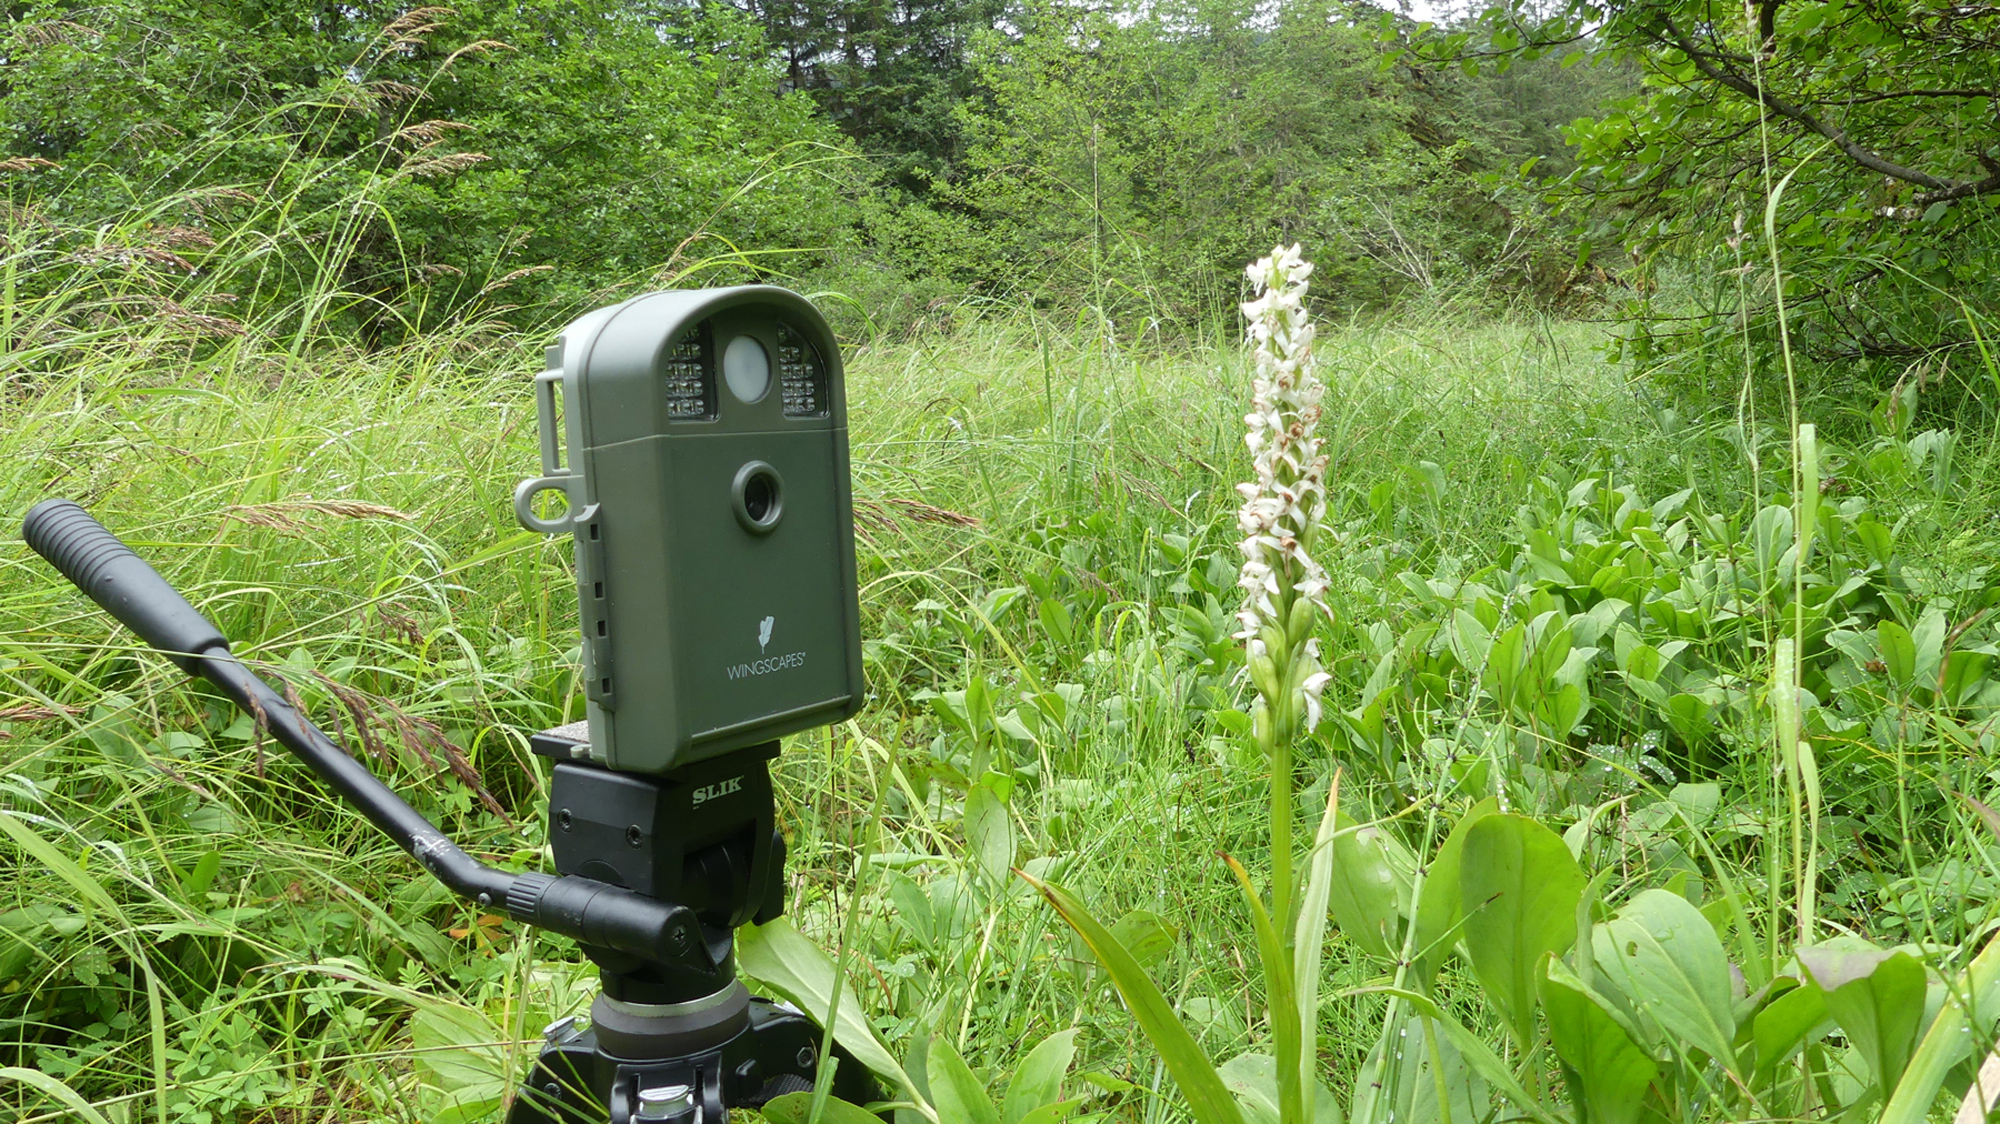
\includegraphics[width=\textwidth]{img/camera.jpg}
\caption{Motion-sensitive trail cam positioned to record visitors to \emph{Platanthera dilatata}.}
\label{camera}
\end{center}
\end{figure} 
\begin{multicols}{2}

\begin{figure}[H]
\begin{center}
%\vspace{2mm}
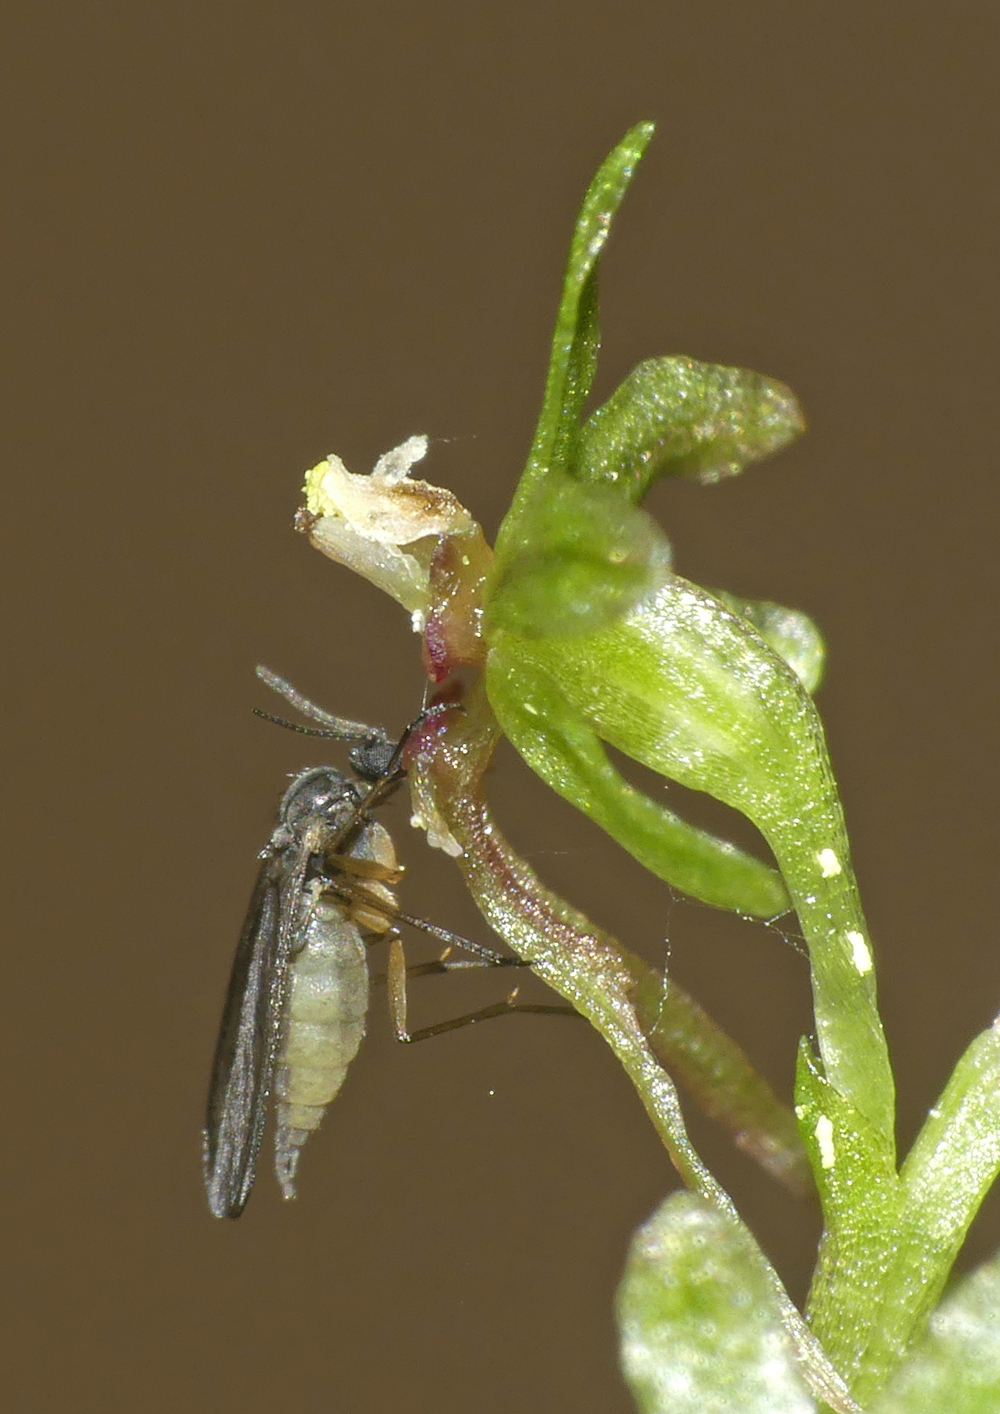
\includegraphics[width=\textwidth]{img/Sciaridae.jpg}
\caption{A dark-winged fungus gnat (Sciaridae) on flowers of the twayblade \emph{Listera cordata}.}
\label{Sciaridae}
\end{center}
\end{figure}

Seven species occupy rainforest habitat. Calypso (\emph{Calypso bulbosa}
var.\ \emph{occidentalis}) is restricted to small forested islands. In
early spring it produces small showy pink slipper-like flowers that lack
a food reward. This orchid is pollinated by queen bumble-bees
(\emph{Bombus} spp.) that switch foraging to other nectar-producing plant
species, resulting in low seed pod production.



Three forest species flower in late spring and early summer, producing
short inflorescences of small green flowers. The heart-leaved twayblade
(\emph{Listera cordata}) and western twayblade (\emph{L.\ banksiana}) are
frequent in old-growth forests, while the blunt-leaved orchid
(\emph{Platanthera obtusata}) is rare in coastal forests. \emph{Listera
cordata} produces nectar at the lip base, and is pollinated by fungus
gnats (Mycetophilidae and Sciaridae) \citep{AckermanMesler1979}.
However, no pollinators are reported for \emph{L.\ banksiana}. \emph{Platanthera
obtusata} has a nectar spur and is pollinated primarily by mosquitoes
(Cuclidae) \citep{Gorham1976}.

\begin{figure}[H]
\begin{center}
\vspace{2mm}
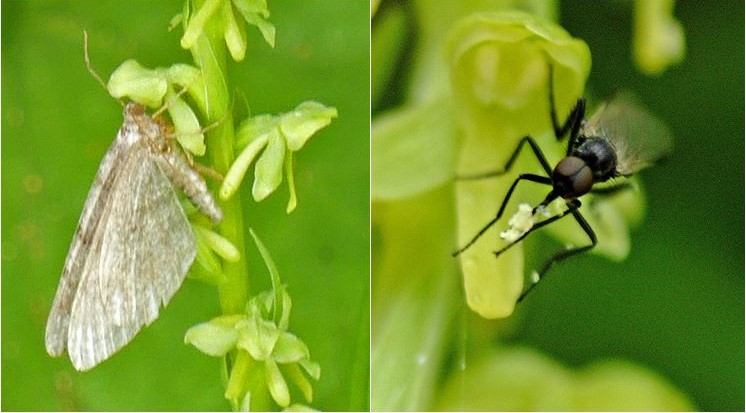
\includegraphics[width=\textwidth]{img/moth_empidid.jpg}
\caption{A geometrid moth (left) and a dance fly (Empididae, right) visiting flowers of \emph{Platanthera stricta}.  Note settling behavior of geometrid and pollinia on proboscis of dance fly.}
\label{moth_empidid}
\end{center}
\end{figure}

\begin{figure}[H]
\begin{center}
\vspace{2mm}
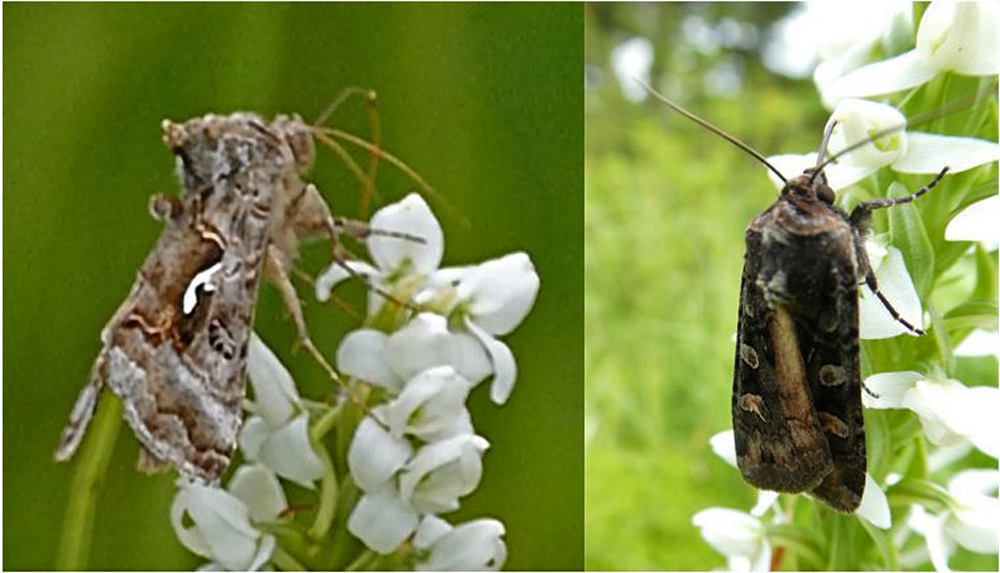
\includegraphics[width=\textwidth]{img/Platanthera_dilatata_Noctuidae.jpg}
\caption{Noctuidae moths foraging on flowers of \emph{Platanthera dilatata}. Note settling behavior, length of proboscis and presence of pollinia.}
\label{Platanthera_dilatata_Noctuidae}
\end{center}
\end{figure}

The early coralroot (\emph{Corallorhiza trifida}) and the western
coralroot (\emph{C.\ mertensiana}) often occur with twayblades in
near-coastal forests. They are less common and tend to flower later,
producing leafless stalks bearing small green and white flowers in
\emph{C.\ trifida} or larger purple and white flowers in \emph{C.\
mertensiana}. \emph{Corallorhiza trifida} has a reduced nectar spur and
has been shown to be autogamous, forming seed pods in exclosures
\citep{Catling1983}. The open structure and longer nectar spur of \emph{C.\
mertensiana} flowers suggest insect pollination \citep{Freudenstein1997};
however, no pollinators are reported. The giant rattlesnake plantain
(\emph{Goodyera oblongifolia}) is restricted to near-coastal forest. It
flowers in late summer, producing a tall spike of white flowers from an
evergreen basal rosette of dark green leaves. Nectar is produced at the
base of a short floral tube, and it is bumble bee
(\emph{Bombus})-pollinated \citep{Ackerman1975}.



Six species occur in muskeg bogs and uplift meadows. The bog adder's
mouth (\emph{Malaxis paludosa}) occupies muskeg, while the Aleutian
adder's mouth (\emph{M.\ diphyllos}) occurs in bogs and meadows. They
produce short spikes of minute green flowers from basal leaves in
mid-summer, and are rare and inconspicuous. Both \emph{Malaxis} species
produce small amounts of nectar at the base of the lip, and are probably
pollinated by fungus gnats \citep[][]{ReevesReeves1984}, though they
have not been confirmed for \emph{M.\ diphyllos}. They can co-occur with
the equally rare Chamisso's orchid (\emph{Platanthera chorisiana}),
which produces short inflorescences bearing small green flowers. This
species is reported as autogamous in Canada \citep{Catling1984}; but, in
Japan it produces nectar in a short spur and is pollinated by the beetle
\emph{Oedemeronia lucidicollis} \citep{Inoue1981}.


\begin{figure}[H]
\begin{center}
\vspace{2mm}
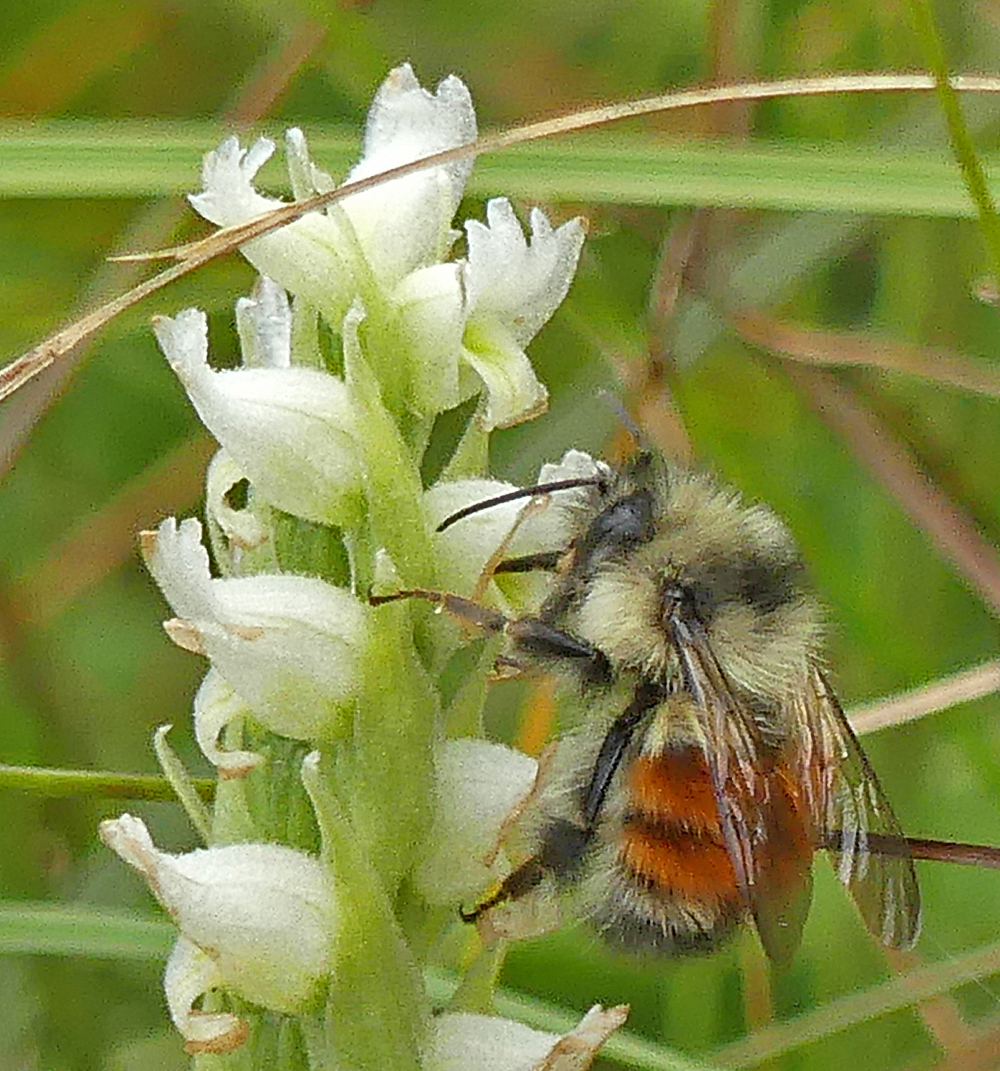
\includegraphics[width=\textwidth]{img/Bombus_melanogynus.jpg}
\caption{The bumble bee \emph{Bombus melanogynus} foraging on \emph{Spiranthes romanzoffiana}.}
\label{Bombus_melanogynus}
\end{center}
\end{figure}


The slender bog orchid (\emph{Platanthera stricta}) occurs in muskeg,
muskeg-forest borders and roadsides. It begins flowering in early
summer, producing tall leafy stalks with spikes of small green flowers
with short nectar spurs. This orchid appears to be a pollinator
generalist, as it is pollinated by moths (Geometridae), dance flies
(Empididae spp.), and \emph{Bombus} species \citep{Pattetal1989}.
The white bog orchid (\emph{Platanthera dilatata} var.\ \emph{dilatata})
grows in open muskeg, meadows, and along roadsides. It begins flowering
in mid-summer, producing tall leafy stalks with spikes of fragrant white
flowers with long nectar spurs. Only Noctuidae moths are reported as
pollinating this species \citep{Larson1992}. Noctuidae are termed settling
moths with respect to \emph{Platanthera} pollination, as they may alight
or partially hover while grasping flowers and do not hover in the same
manner as Sphingidae \citep{HapemanInoue1997}. These longer-tongued hawk
moths have been suggested as pollinators as well, especially of \emph{P.\
dilatata} var.\ \emph{leucostachys}, which has longer nectar spurs than the
typical variety \citep{Sheviak2002}. The ladies' tresses orchid
(\emph{Spiranthes romanzoffiana}) flowers in late summer in muskeg and
along lakeshores. Although less common, it often occurs with \emph{P.\
dilatata}; its inflorescences reach maturity as those of the latter
species are senescing. It produces a short spike of fragrant white
flowers with nectar at the base of the floral tube, and is pollinated by
\emph{Bombus} spp.\ \citep{LarsonLarson1987}.

\begin{figure}[H]
\begin{center}
\vspace{2mm}
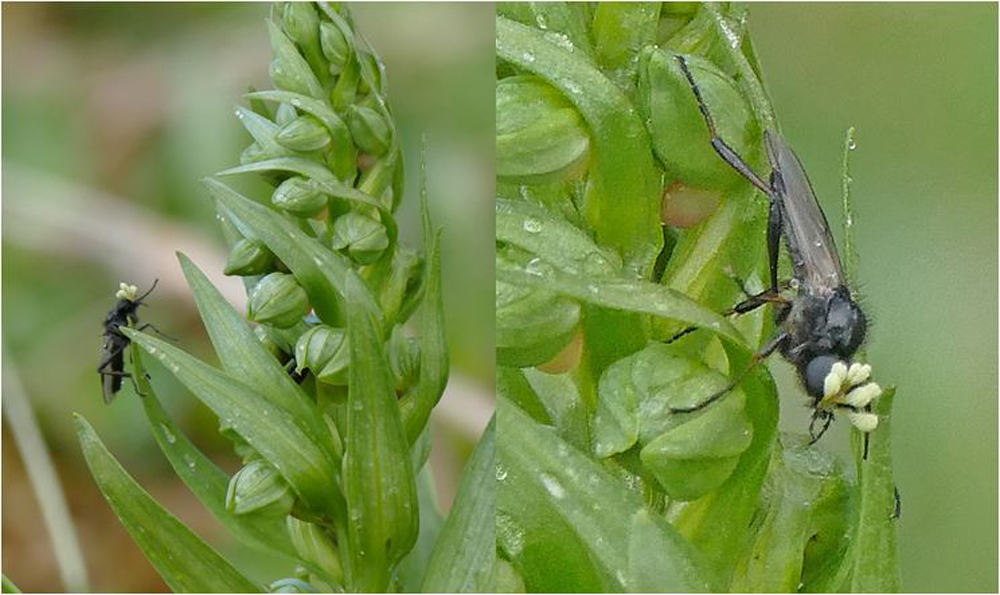
\includegraphics[width=\textwidth]{img/Bibionidae.jpg}
\caption{A March fly (Bibionidae) pollinating \emph{Coeloglossum viride}.  Note pollinia at the front of the head and partly opened flowers.}
\label{Bibionidae}
\end{center}
\end{figure}



\section{Methods}

Much of this work was conducted using motion-sensitive or time-lapse
trail cams with flash and close focus capabilities. They could be left
unattended to determine, and sometimes quantify, diurnal and nocturnal
visitation by insects that were sensitive to human presence (Figure \ref{camera}).
We also recorded video, time-lapse and other photographic images on
still cameras with macro capabilities. A blacklight was used to capture
moths foraging on \emph{Goodyera oblongifolia}. Links to videos and
slides from this work are provided in the \hyperref[videos]{videos and slide shows} section (page \pageref{videos}). The working conditions
for this project were not conducive for collecting voucher insect
specimens. Often only a single individual was observed carrying
pollinia, and its collection would have disrupted pollination. Many
other visitors were observed only in video camera outputs, and could not
be accessed for precise identification. As a result, we relied upon
field observation or identification from photographs for species
identities, and many pollinators could not be identified below the
family level. For several orchid species, we used insect exclosures to
determine whether they were autogamous, and we also quantified seed pod
production to assess the effectiveness of pollinators.

\begin{figure}[H]
\begin{center}
\vspace{2mm}
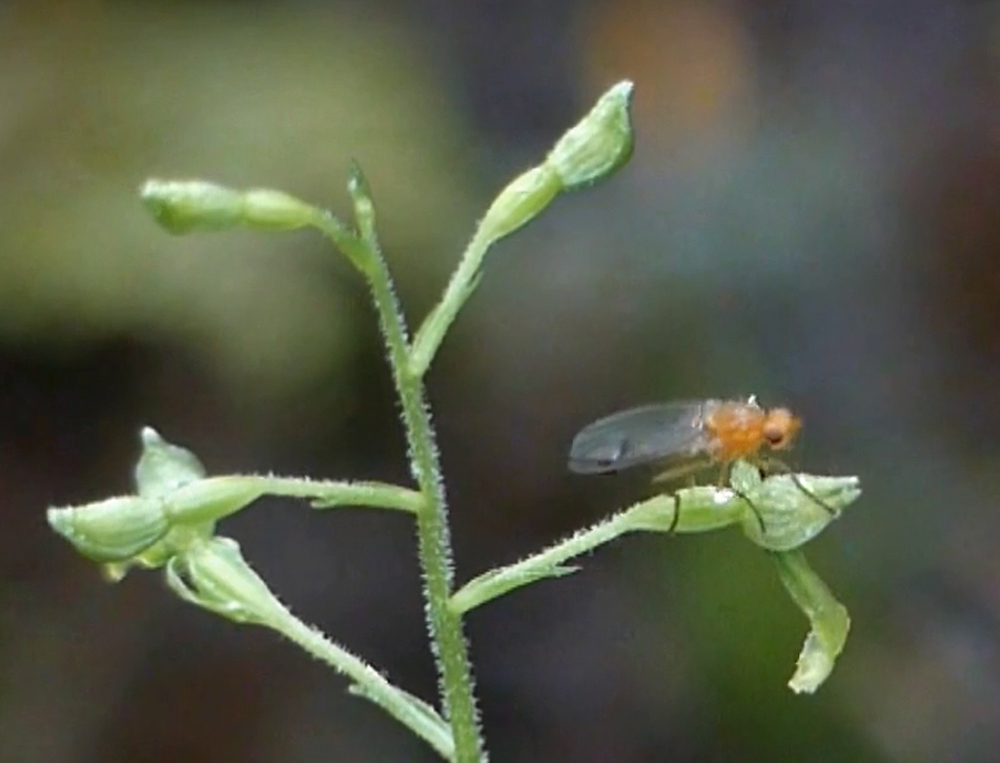
\includegraphics[width=\textwidth]{img/Listera_banksiana_Dryomyza.jpg}
\caption{A \emph{Dryomyza} fly (Dryomyzidae) on flower of \emph{Listera banksiana}.}
\label{Listera_banksiana_Dryomyza}
\end{center}
\end{figure} 


\begin{figure}[H]
\begin{center}
\vspace{2mm}
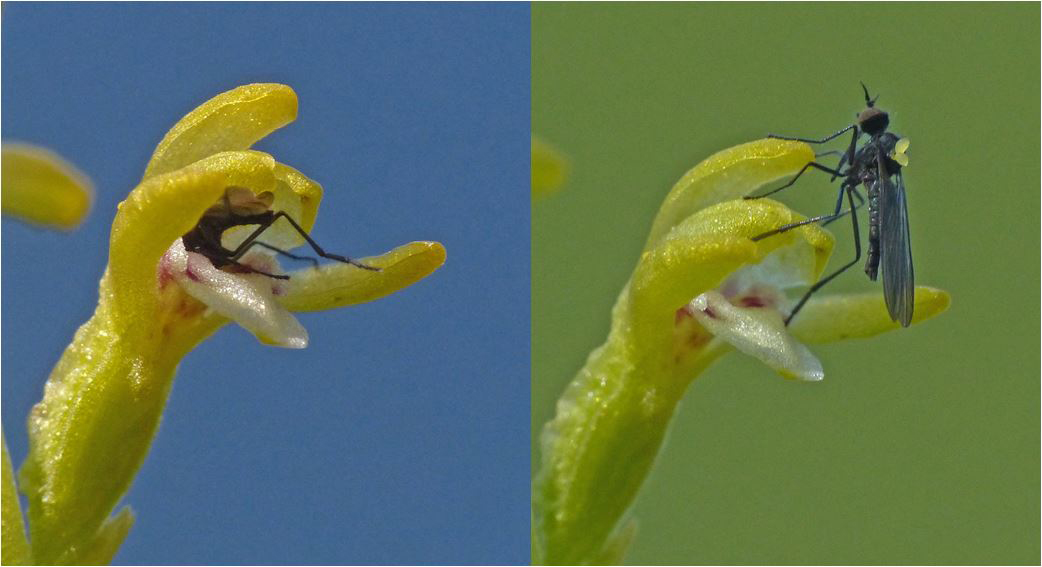
\includegraphics[width=\textwidth]{img/Corallorhiza_trifida_Empididae.jpg}
\caption{Sequence showing a dance fly (Empididae) entering and leaving a flower of \emph{Corallorhiza trifida} while bearing pollinia on its thorax.}
\label{Corallorhiza_trifida_Empididae}
\end{center}
\end{figure}

\section{Results and Discussion}

We observed 15 or more insect taxa visiting ten orchid species that were
either pollinators or appeared likely to be pollinators (Table \ref{pollinatortable}). They
represented the Hymenoptera, Lepidoptera, and Diptera. These insects
represented five of the seven taxa reported in the North America
literature as pollinators and about eight newly recorded pollinators for
the study orchids. The Noctuidae were particularly difficult to identify
as species. Other insects included one pollen consumer and two nectar
thieves \citep{Inouye1980}, which consistently visited some orchid species.
At least four spider taxa occurred on the orchids, including three
web-spinning species and one ambushing species, as well as several
predatory wasp species.

\subsection{Confirmation of reported pollinators}

Among forest species, fungus gnats were observed repeatedly on
\emph{Listera cordata}; however, none were bearing pollinia. One species
(Figure \ref{Sciaridae}) appears to be a dusky-winged fungus gnat (Sciaridae).
We made a single observation of a \emph{Bombus} species visiting \emph{Goodyera
oblongifolia}.


\begin{figure}[H]
\begin{center}
\vspace{2mm}
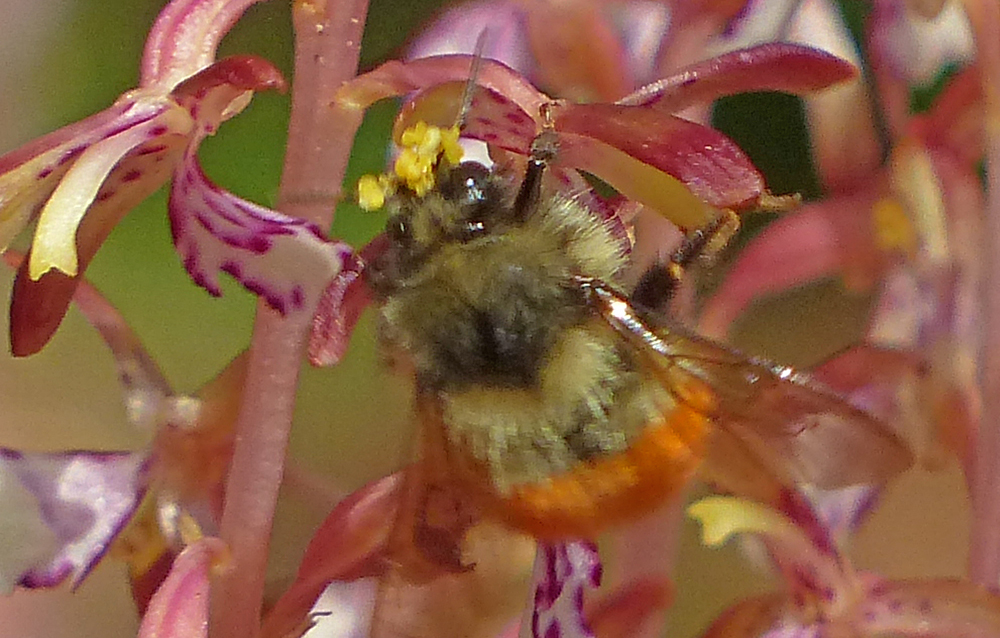
\includegraphics[width=\textwidth]{img/Corallorhiza_mertensiana_Bombus.jpg}
\caption{\emph{Bombus} species pollinating \emph{Corallorhiza mertensiana}. Note pollinia positioned below eyes.}
\label{Corallorhiza_mertensiana_Bombus}
\end{center}
\end{figure}

In fen, meadow and muskeg habitats, we recorded pollinators on
three orchid species. On \emph{Platanthera stricta} we observed a
dance fly (Empididae sp.) bearing pollen on its proboscis as well
as a moth species (Geometridae) foraging for nectar (Figure \ref{moth_empidid}). On
\emph{Platanthera dilatata, several Noctuidae moth species
(probably \emph{Autographa corusca} and \emph{Actebia fennica}}) were
found bearing pollinia on their tongues while foraging for nectar
(Figure \ref{Platanthera_dilatata_Noctuidae}). On \emph{Spiranthes romanzoffiana}, we recorded visits by
the black-tailed bumble bee (\emph{Bombus melanogynus}) (Figure \ref{Bombus_melanogynus}). As
this orchid flowers in late summer, they were probably male drones.
\emph{Goodyera oblongifolia} is also late-flowering, and may have been
visited by this \emph{Bombus} species as well.





\subsection{Newly reported pollinators or visitors}

In alpine, \emph{Coeloglossum viride} was pollinated by march flies
(Bibionidae, possibly \emph{Bibio vestitus}). These flies entered and
exited flowers while bearing multiple pollinia at the base of their
heads below the eyes (Figure \ref{Bibionidae}). They often force into newly opening
flowers, apparently to access nectar. This insect appears to be an
important pollinator of this orchid in the alpine zone of our study
area. More work is needed to determine whether additional insects, such
as those in European alpine, pollinate this species in North America.

\begin{figure}[H]
\begin{center}
\vspace{2mm}
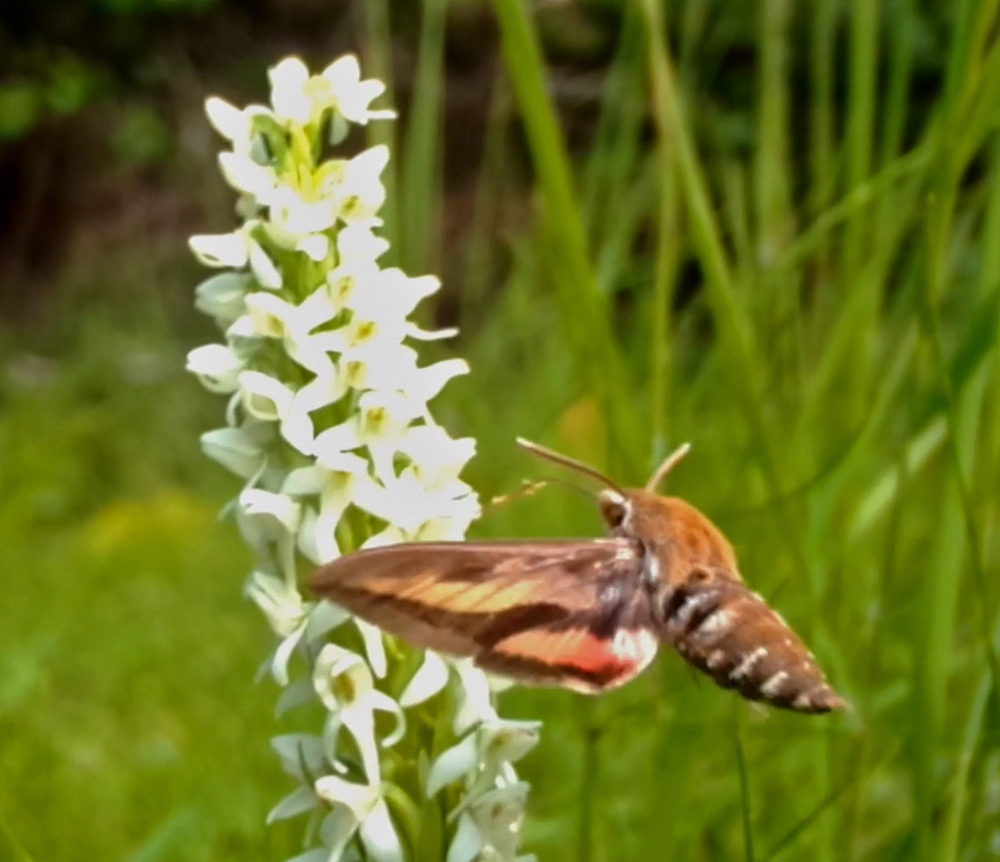
\includegraphics[width=\textwidth]{img/Platanthera_dilatata_Hyles_galii.jpg}
\caption{The hawkmoth \emph{Hyles gallii} pollinating \emph{Platanthera dilatata}. Note hovering behavior and pollinia on the proboscis.}
\label{Platanthera_dilatata_Hyles_galii}
\end{center}
\end{figure}

\begin{figure}[H]
\begin{center}
\vspace{2mm}
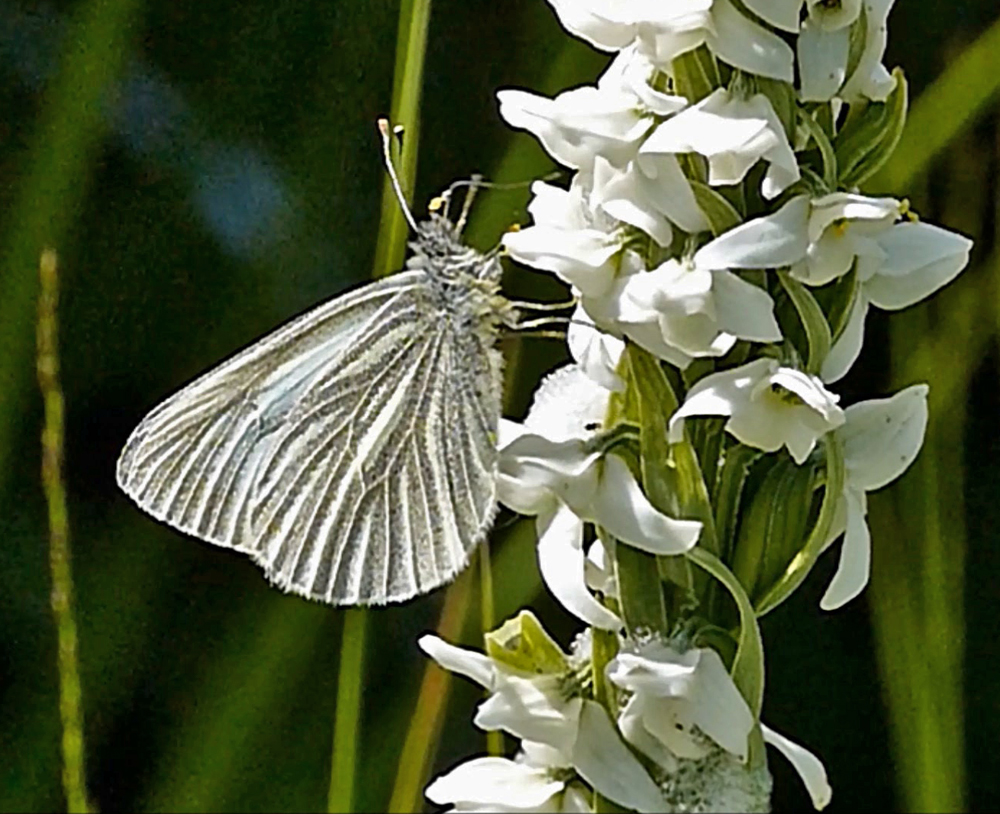
\includegraphics[width=\textwidth]{img/Platanthera_dilatata_Pieris_marginalis.jpg}
\caption{The butterfly \emph{Pieris marginalis} nectaring on \emph{Platanthera dilatata}.  Note pollinia on proboscis.}
\label{Platanthera_dilatata_Pieris_marginalis}
\end{center}
\end{figure}


In forest habitats we recorded new pollinators (or apparent
pollinators), for three orchid species. Although no pollinators or other
insect visitors have been reported for \emph{Listera banksiana}, we
observed \emph{Dryomyza} flies (\emph{Dryomyza} sp.) visiting this orchid
(Figure \ref{Listera_banksiana_Dryomyza}). They appeared to be foraging for a food reward on the orchid
lip; however, none of the insects were observed carrying pollinia. The
\emph{Dryomyza} fly oviposits on bear scat and salmon carcasses, and might be
attracted to this orchid if it emits a similar odor. Most individuals of
\emph{L.\ banksiana} produced seed pods, and those we excluded from
pollinators did not produce seed pods. This suggests that \emph{L.\
banksiana} is obligately insect-pollinated; but, more work is needed to
confirm pollinating species. Although \emph{Corallorhiza trifida} may be
autogamous, we observed dance flies (Empididae sp.) entering their
flowers and exiting bearing pollinia on their upper thorax (Figure \ref{Corallorhiza_trifida_Empididae}).
These visits could provide occasional outcrossing in this apparently
self-pollinating orchid. Dance flies were also observed probing flowers
of \emph{Platanthera obtusata} but did not extract pollinia and may not
pollinate this species. Nevertheless, they appear to be versatile
pollinators as one was observed bearing pollinia from \emph{Platanthera
stricta} on its proboscis. We recorded pollination of \emph{Corallorhiza
mertensiana} by a \emph{Bombus} species. Multiple pollinia were
deposited at the base of the head below the eyes of this bee while it
foraged for nectar (Figure \ref{Corallorhiza_mertensiana_Bombus}). Our data suggest that bees may be
efficient pollinators of this coralroot. Open-pollinated plants at two
sites averaged 50--80\% of flowers forming seed pods, while
inflorescences that were bagged to exclude pollinators did not produce
seed pods. This suggests that \emph{C. mertensiana} is an obligate
insect-pollinated species.



\begin{figure}[H]
\begin{center}
\vspace{2mm}
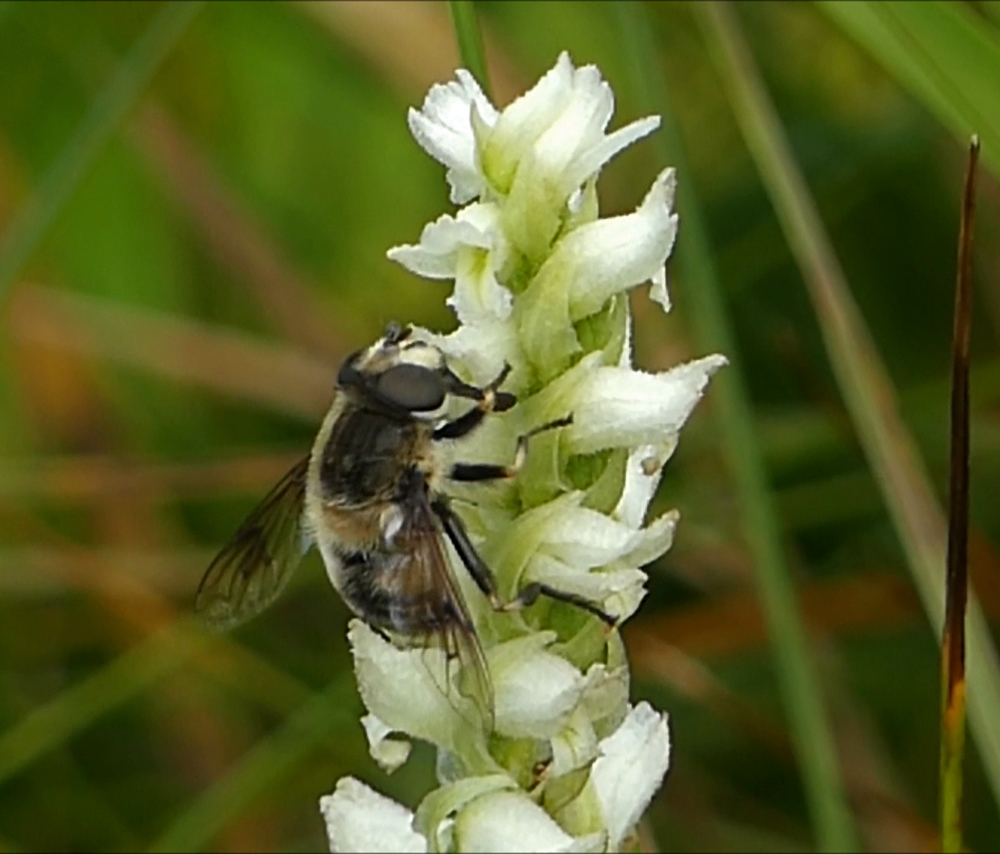
\includegraphics[width=\textwidth]{img/Spiranthes_romanzoffiana_Eristalis_anthophorina.jpg}
\caption{The bee-mimic \emph{Eristalis anthophorina} foraging on \emph{Spiranthes romanzoffiana}.}
\label{Spiranthes_romanzoffiana_Eristalis_anthophorina}
\end{center}
\end{figure}



In muskeg and meadow habitats, we recorded new pollinators for two
species. In addition to expected visits by Noctuidae moth species, we
recorded diurnal and nocturnal visits by the hawkmoth \emph{Hyles
gallii} to \emph{Platanthera dilatata} (Figure \ref{Platanthera_dilatata_Hyles_galii}). In contrast to the
low number of pollinia carried by Noctuidae, \emph{H.\ gallii} carried
large numbers of pollinia on its proboscis. It appeared to be a very
efficient pollinator even though its proboscis length greatly exceeded
nectar spur length. We also observed occasional visits by the margined
white butterfly (\emph{Peris marginalis}) to this orchid, during which
it extracted pollinia on its proboscis (Figure \ref{Platanthera_dilatata_Pieris_marginalis}). This butterfly may
be a rare and inefficient pollinator of \emph{P.\ dilatata} in our
region. \emph{Bombus} species also occasionally visited this orchid, but it is
unlikely that they were able to access nectar held in its comparatively
long nectar spurs. We suggest that as with \emph{P.\ stricta},
\emph{P.\ dilatata} is a generalist with regard to pollinators, but that
they vary in pollination efficiency. Although \emph{Spiranthes
romanzoffiana} is reported as bee-pollinated, we also observed a
bee-mimic Syrphidae (\emph{Eristalis anthophorina}) on this orchid. It
foraged in the same manner as \emph{Bombus} species by moving upward on
the inflorescence while probing flowers with its proboscis (Figure \ref{Spiranthes_romanzoffiana_Eristalis_anthophorina}).
Although we could not detect presence of pollinia on its proboscis, it
may function as a pollinator.




\begin{figure}[H]
\begin{center}
\vspace{2mm}
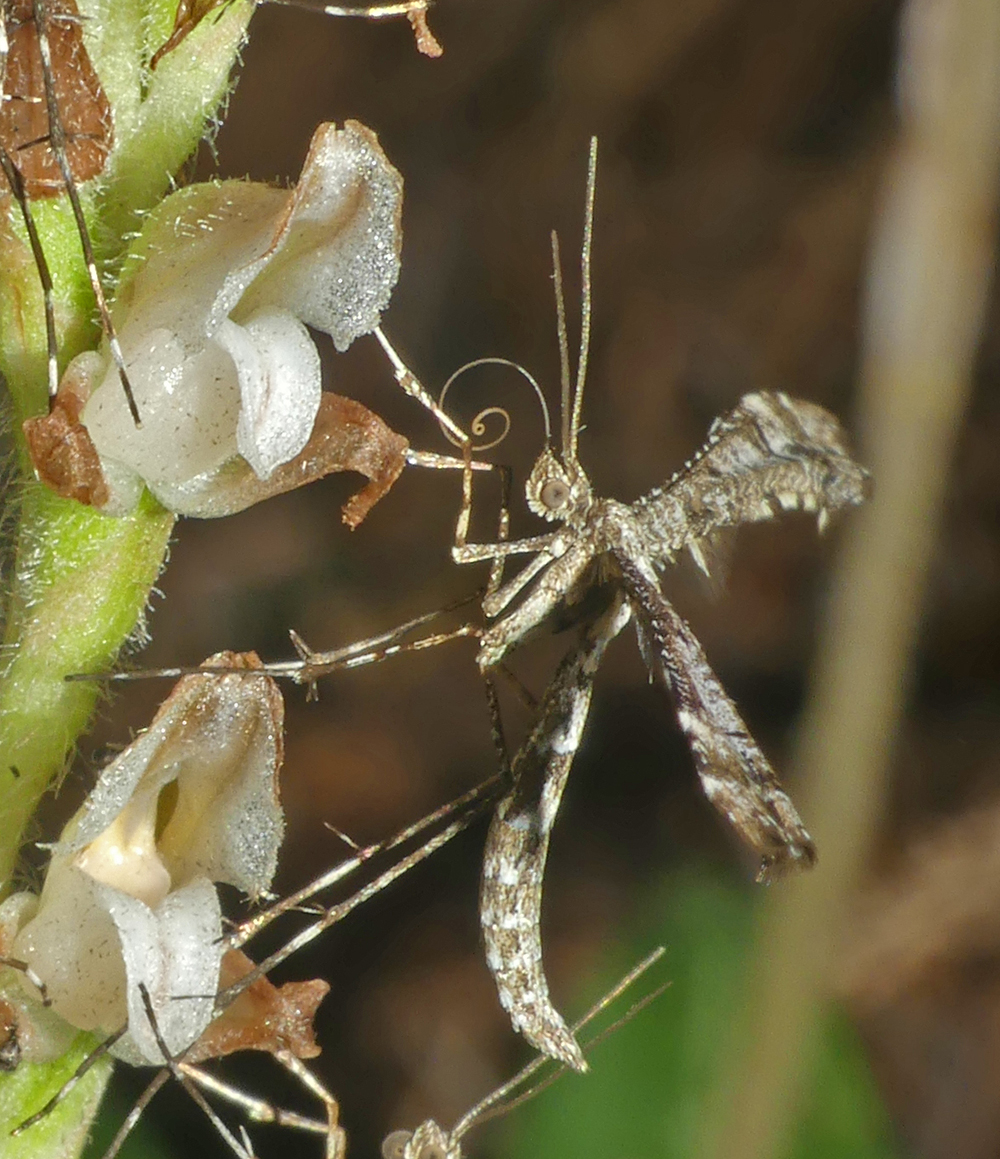
\includegraphics[width=\textwidth]{img/Goodyera_oblongifolia_Amblyptilia_pica.jpg}
\caption{The plume moth \emph{Amblyptilia pica} foraging on \emph{Goodyera oblongifolia}. Note slender proboscis relative to size of floral tube.}
\label{Goodyera_oblongifolia_Amblyptilia_pica}
\end{center}
\end{figure}




\subsection{Nectar thieves}

Species belonging to two different families appeared to function as
nectar thieves on \emph{Goodyera oblongifolia}. In early fall, numerous
geranium plume moths (\emph{Amblyptilia pica}) were observed visiting
late-flowering plants of \emph{G.\ oblongifolia} (Figure \ref{Goodyera_oblongifolia_Amblyptilia_pica}). These
insects easily inserted their long slender proboscis into the
comparatively short floral tube of the orchids. None were observed
bearing pollinia, and the plants they visited did not produce seed pods.
This species overwinters as an adult, and the nectar from \emph{G.\
oblongifolia} may be quite beneficial to these insects, as no other
flowering plant species occurred in the area occupied by the orchids. We
have observed such visitation at multiple sites over multiple years. We
also observed a plume moth (\emph{Amblyptilia} sp.) nectaring on \emph{P.\
dilatata} without removing pollinia. Likewise, \emph{A.\ pica} has been
recorded as a probable nectar thief on \emph{P.\ orbiculata} in New
Hampshire \citep{Bergumetal2018}.


\begin{figure}[H]
\begin{center}
\vspace{2mm}
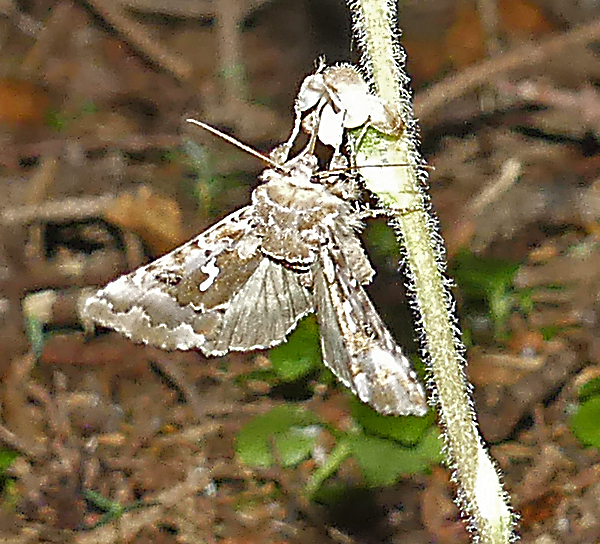
\includegraphics[width=\textwidth]{img/Goodyera_oblongifolia_Noctuidae.jpg}
\caption{Nocturnally foraging \emph{Autographa corusca} on \emph{Goodyera oblongifolia}.  Note proboscis inserted into floral tube.}
\label{Goodyera_oblongifolia_Noctuidae}
\end{center}
\end{figure}



\emph{Goodyera oblongifolia} was also visited by a second apparent
nectar thief, Noctuidae moths that may be \emph{Autographa corusca}
(Figure \ref{Goodyera_oblongifolia_Noctuidae}). Over a fifteen day period, 24 hour time-lapse videos (at
one minute intervals) revealed an average of 8.7 visits per night
among 15 plants. However, no diurnal visitors were recorded, and no seed
pods were formed on these plants. In an area 0.15~km away where plants
were not video monitored, 62\% of 178 flowers produced seed pods among
17 plants. Although we do not know if Noctuidae visited the adjacent
area, they did not pollinate plants at the first site, and their
repeated visits suggest that they were removing nectar from these
plants. Their proboscis length is greater that the floral tube, which
may have facilitated nectar thievery. Several of these moths that were
captured by blacklight also did not bear pollinia. \emph{Goodyera
oblongifolia} is reported to have naturally low levels of seed pod
production, and spreads by rhizomes \citep{Ackerman1975}. Nectar thieves can
influence reproductive fitness by influencing behavior of pollinators
\citep{Zhangetal2014}. If the high visitation rate we observed for
Noctuidae species reduced nectar availability, it might have contributed
to reduced visitation by \emph{Bombus} and the low reproduction that we
observed. If widespread, this process could provide selective pressure
for the development of vegetative spread as an alternate use of
reproductive resources by \emph{G.\ oblongifolia}. More work is needed to
test this hypothesis.

\begin{figure}[H]
\begin{center}
\vspace{2mm}
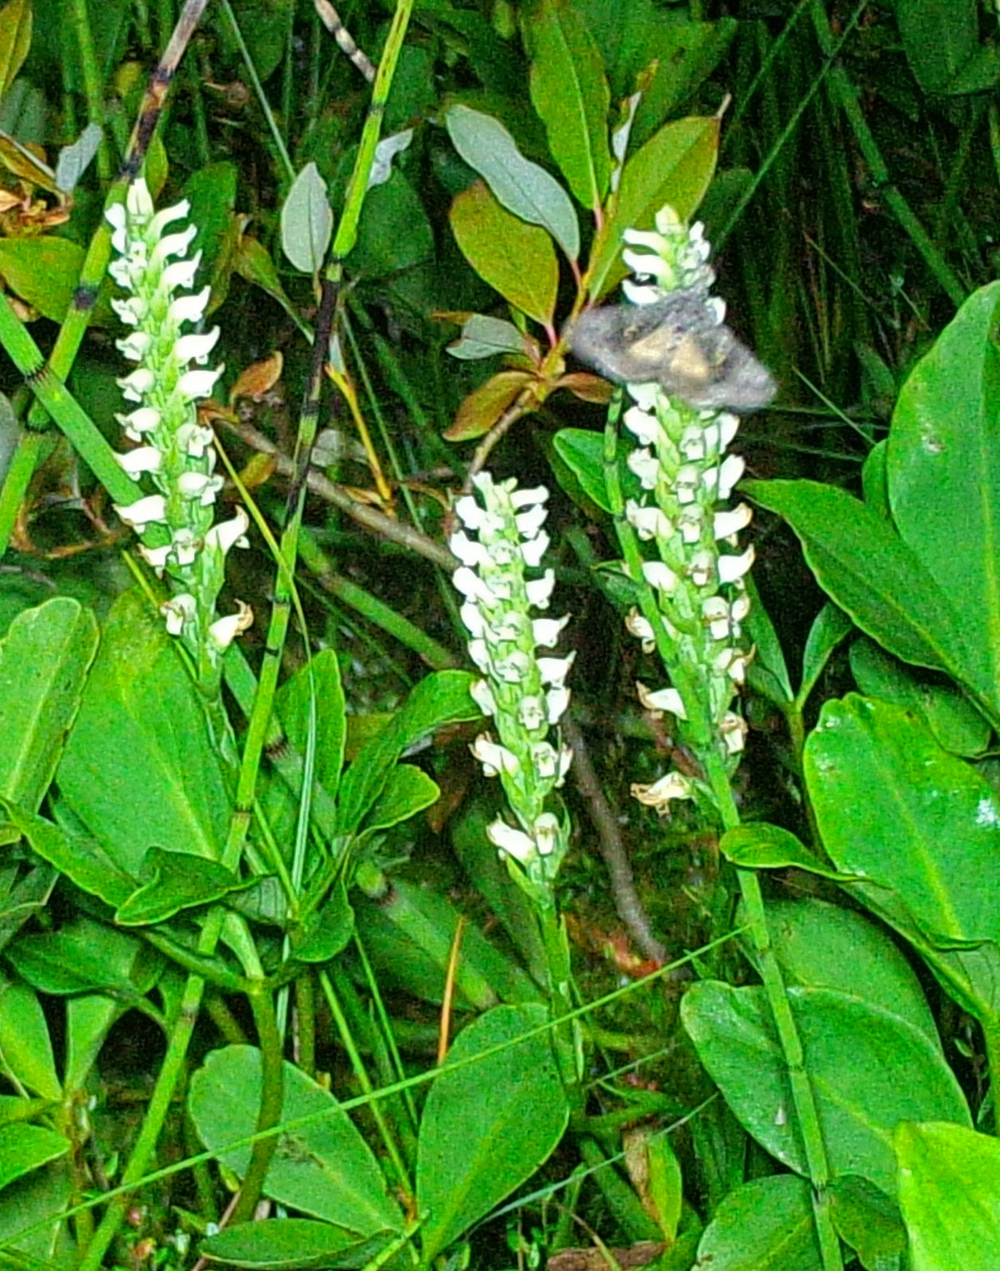
\includegraphics[width=\textwidth]{img/Spiranthes_romazoffiana_Noctuidae.jpg}
\caption{Nocturnally foraging Noctuidae on \emph{Spiranthes romanzoffiana}.}
\label{Spiranthes_romazoffiana_Noctuidae}
\end{center}
\end{figure}


We also video-recorded nocturnal visits by Noctuidae moths to a second
\emph{Bombus}-pollinated orchid, \emph{Spiranthes romazoffiana} (Figure
\ref{Spiranthes_romazoffiana_Noctuidae}). This orchid is closely related to \emph{Goodyera}, and Noctuidae
species may function as nectar thieves on this species as well. However,
it differs from \emph{G.\ oblongifolia} by having relatively high levels
of \emph{Bombus} visitation and seed pod production \citep{LarsonLarson1987}. The greater level of reproduction for \emph{S.\ romanzoffiana} could be related to habitat conditions, as this
orchid occurs in open vegetation where its inflorescences may be highly
visible \citep{LarsonLarson1990}, while coastal \emph{G.\ oblongifolia} populations occupy dense shaded spruce forests
\citep{Ackerman1975}.





Although not reported in the literature, our results indicate that
Noctuidae species that pollinate \emph{Platanthera dilatata} may
function as nocturnal nectar thieves on two \emph{Bombus}-pollinated
orchid species with overlapping flowering periods. \emph{Platanthera
dilatata} flowers from late June through late July in our region, while
\emph{Spiranthes romanzoffiana} and \emph{Goodyera oblongifolia} usually
flower from mid-July through August. More work is needed to determine
the number of Noctuidae species involved in visitation to these orchids
and whether individual Noctuidae species overlap in their visits. The
Noctuidae species we have observed appear to have proboscis lengths that
exceed the nectar spur length of \emph{P.\ dilatata} as well as the
floral tube lengths of \emph{S.\ romanzoffiana} and \emph{G.\
oblongifolia}. However, these species differ in their manner of pollinia
placement \citep{Argue2012a, Argue2012b}. % Need to ask which of the Argue references this came from.
\emph{Platanthera dilatata} positions its
pollinia on either side of the nectar spur entrance, which facilitates
pollinia deposition on the proboscis. The latter species position their
pollinia within the floral tube on its dorsal side, which are attached
to the proboscis of nectar-seeking species. The pollinia may be less
likely to contact the slender proboscis of Noctuidae moths (Figure \ref{Goodyera_oblongifolia_Noctuidae}).
Also, as their flowers mature, the pollinia are moved upward to expose
the stigma \citep{Argue2012a, Argue2012b}. % Need to ask which of the Argue references this came from.
In \emph{G.\ oblongifolia,} the pollinia lose
their adhesive ability as the flower matures, making them less likely to
adhere to an insect proboscis.

\subsection{Pollinator network}

The orchids and insect visitors in our study area comprise a complex
network in which orchids may have multiple pollinators or may share
pollinators and nectar thieves (Figure \ref{pollinator_network}). To some extent, pollinator
types appear to be structured among different orchid groups. For
example, orchids with smaller flowers and more easily accessible nectar
resources display adaptation to Diptera species that have comparatively
small bodies and short tongues. In contrast, orchids with more showy
larger flowers that maintain nectar in recessed spurs show adaptation to
Lepidoptera species. Moreover, proboscis lengths of \emph{Platanthera}
pollinators in this network correspond to orchid nectar spur lengths,
supporting the idea that orchids partition pollinator resources by
adapting their spur lengths to proboscis lengths \citep{HapemanInoue1997}. \emph{Bombus} species, which have intermediate proboscis lengths, visit
orchids with intermediate flower sizes and nectar resources maintained
in shorter floral tubes or nectar spurs. One species, \emph{Calypso
bulbosa}, attracts \emph{Bombus} species by advertising a false reward.
Longer-tongued \emph{Bombus} species that would access greater floral
diversity may occur in our area, but we have no information on this
group. The additional pollinator-nectar thief relationship among the
Lepidoptera-pollinated \emph{Platanthera dilatata} and the
\emph{Bombus}-pollinated \emph{Goodyera oblongifolia} and
\emph{Spiranthes romanzoffiana} suggests that interactions become more
complex in association with larger orchids with greater nectar
resources. However, we may lack comparative information on interactions
among the smaller orchids and pollinators.


\begin{figure}[H]
\begin{center}
\vspace{2mm}
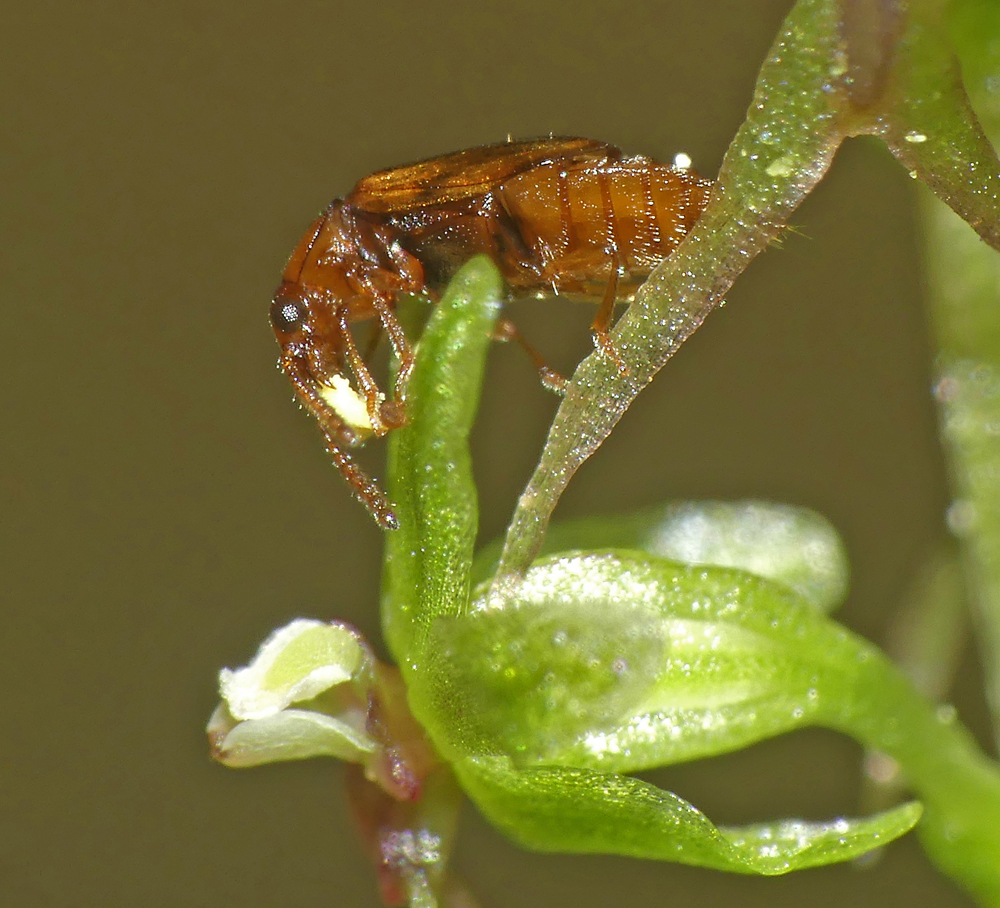
\includegraphics[width=\textwidth]{img/Listera_cordata_Eusphalerum_pothos.jpg}
\caption{The rove beetle \emph{Eusphalerum pothos} consuming pollen of \emph{Listera cordata}.}
\label{Listera_cordata_Eusphalerum_pothos}
\end{center}
\end{figure}

\subsection{Pollen consumers}

A rove beetle species (\emph{Eusphalerum pothos}) was recorded consuming
pollen on the twayblade orchid \emph{Listera cordata} (Figure \ref{Listera_cordata_Eusphalerum_pothos}). Rove
beetles are well known pollenophagous feeders \citep{Sayersetal2019}.
Although we have limited data, we found no difference in seed pod
production between plants attacked by rove beetles and those that did
not have rove beetles. While foraging for pollen, these beetles
occasionally had pollinia attached to their heads, but they did not
appear to pollinate plants.

\subsection{Insect predation}

We observed insect predation by four different spider taxa. However,
predation of pollinators appeared to be rare. Three web-spinning
spiders, the silver long-jawed orb weaver (\emph{Tetragnatha
laboriosa}) and the six-spotted orb weaver (\emph{Araniella
displicata}) were observed on the slender bog orchid (\emph{Platanthera
stricta}). The former species had captured a biting midge
(Ceratopogonidae), while the latter species appears to have captured a wasp (Hymenoptera) % sawfly (Tenthredinidae) 
as a prey item (Figure \ref{Araniella_displicata_Hymenoptera}). As this orchid can occupy muskeg borders where
shrubs are present, this may have facilitated web building by these
spiders. A cobweb spider (Theridiidae) was observed with a captured
fungus gnat on the western twayblade (\emph{Listera cordata}) (Figure
\ref{Theridiidae_Sciaroidea}). This orchid routinely produces a large number of seed pods in our
area, and it is unlikely that pollinator predation affects its levels of
seed production.

\begin{figure}[H]
\begin{center}
\vspace{2mm}
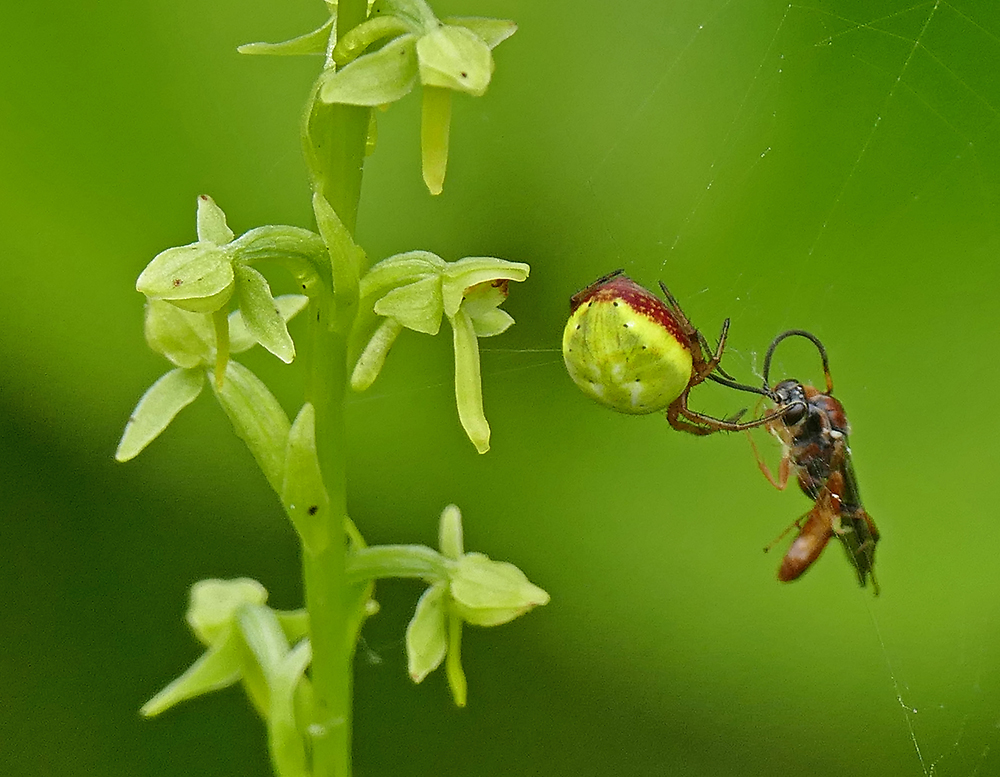
\includegraphics[width=\textwidth]{img/Araniella_displicata_Hymenoptera.jpg}
\caption{The orb weaver \emph{Araniella displicata} with captured wasp on \emph{Platanthera stricta}.}
\label{Araniella_displicata_Hymenoptera}
\end{center}
\end{figure}


\begin{figure}[H]
\begin{center}
\vspace{2mm}
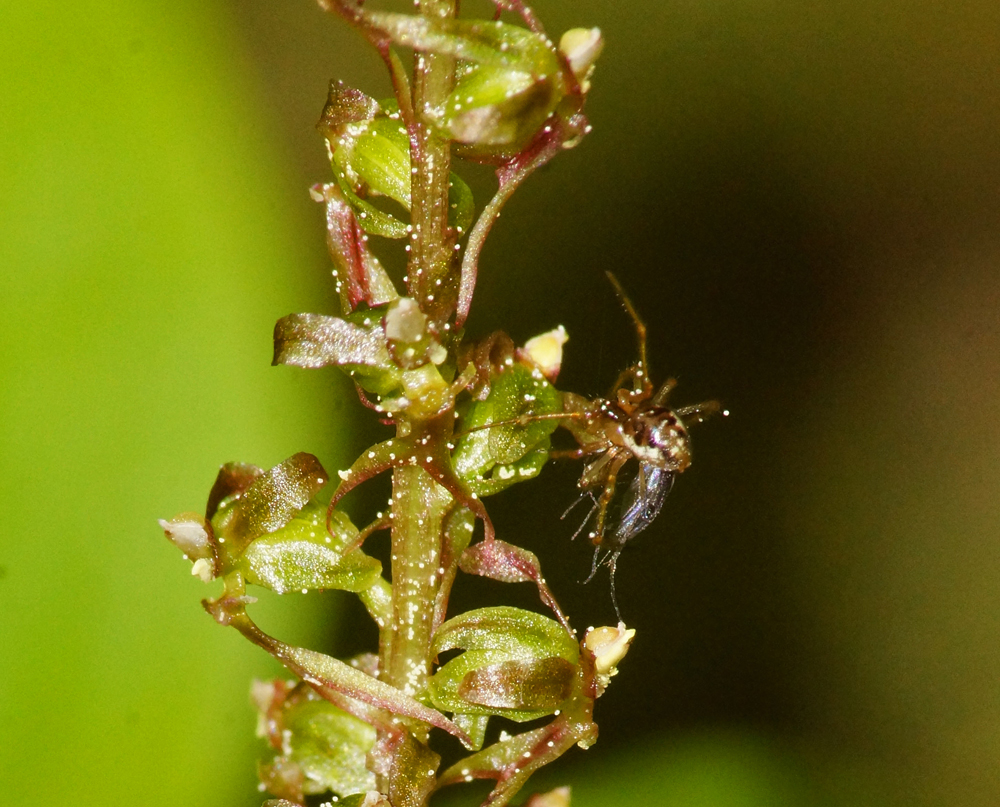
\includegraphics[width=\textwidth]{img/Theridiidae_Sciaroidea.jpg}
\caption{A cobweb spider (Theridiidae) with fungus gnat prey item on \emph{Listera cordata}.}
\label{Theridiidae_Sciaroidea}
\end{center}
\end{figure}


\end{multicols}
\begin{figure}[H]
\begin{center}
\vspace{2mm}
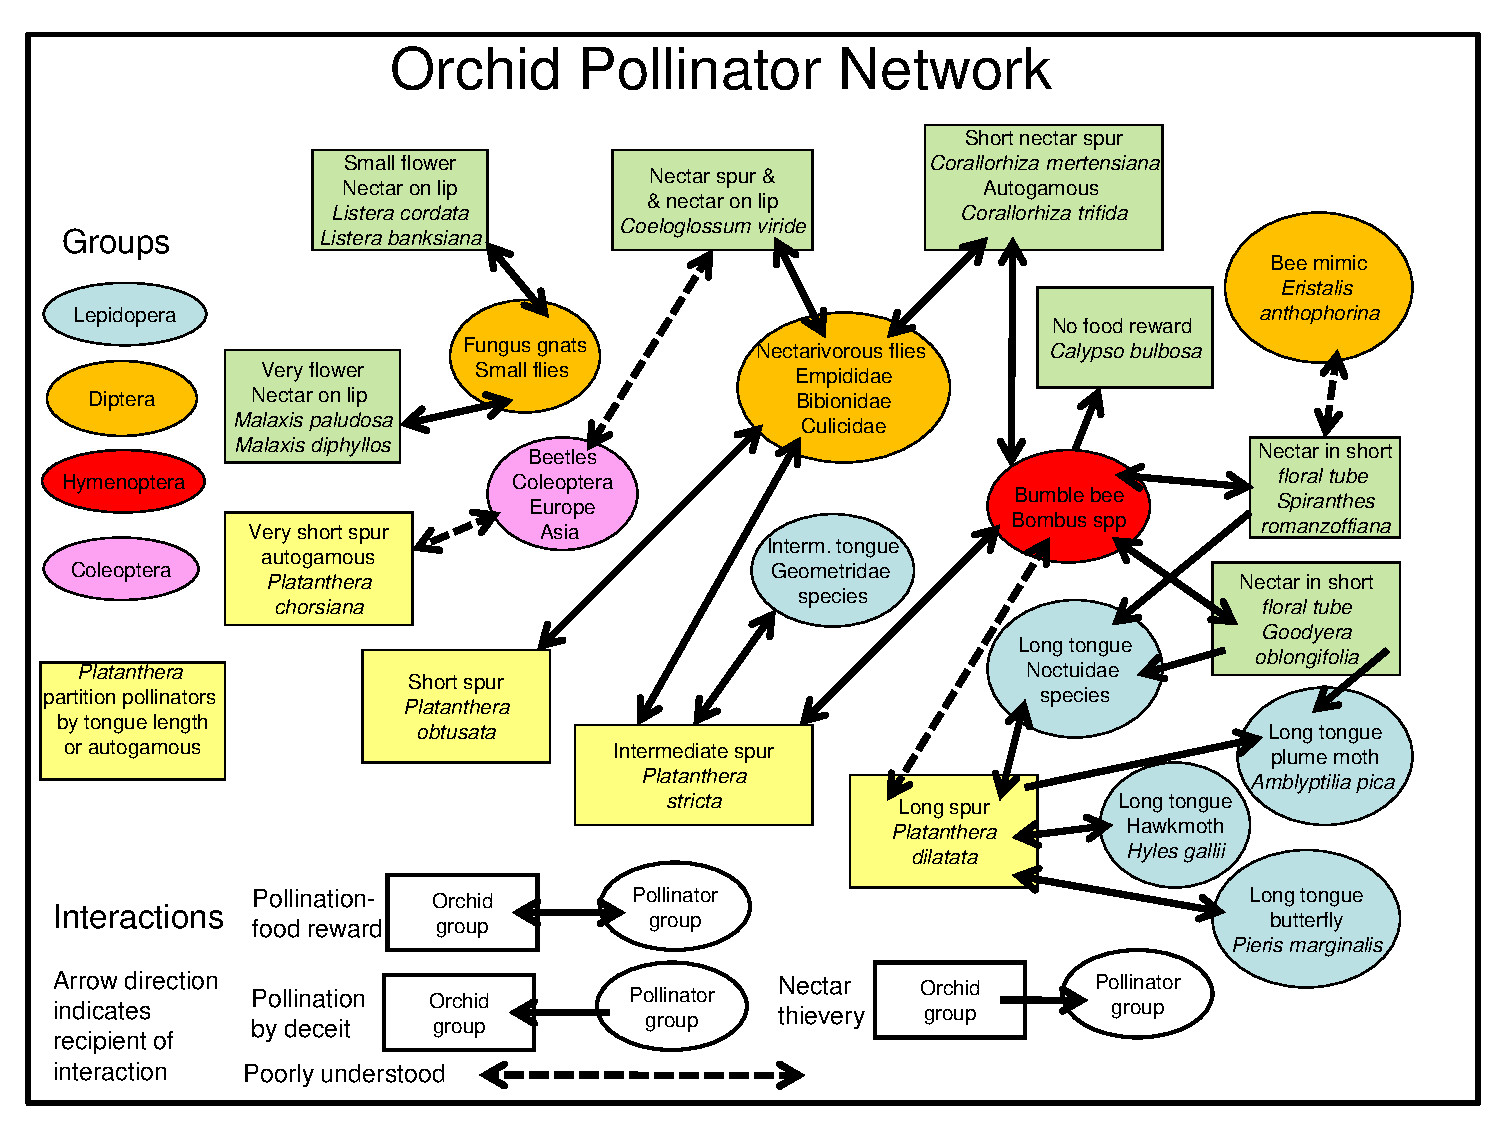
\includegraphics[width=\textwidth]{img/pollinator_network.pdf}
\caption{Relationships in an orchid pollinator network in the Juneau area of Southeast Alaska.  Squares represent orchid species or species groups with similar morphological features.  The \emph{Platanthera} group is color-coded. Circles represent insect pollinators, or pollinator groups with similar morphological features, which are color coded by order.  Arrow directions represent recipients of plant-pollinator interactions.  Double-headed arrows indicate both pollination and food reward, single headed arrows indicate either pollination or food reward by nectar thievery.  Dashed arrows indicate poorly understood relationships due to lack of information.  Tongue is used interchangeably for proboscis in labeling modules.}
\label{pollinator_network}
\end{center}
\end{figure} 
\begin{multicols}{2} 













Crab Spiders (Thomisidae) which hunt by ambushing prey on flowers, were
observed on \emph{Platanthera dilatata}. Their prey included a biting
midge, crane fly (Tipulidae), and horse fly (Tabanidae) (Figure \ref{Misumena_vatia_Tabanidae}).
None of these insects are known pollinators of \emph{Platanthera}
species and it is unknown whether crab spiders impact true pollinators
of these orchids.




Yellow jackets (Vespinae) are occasional visitors to \emph{Platanthera
dilatata}. We do not know whether they are foraging for insect prey, or
perhaps seeking nectar. An Ichneumonid wasp (Ichneumonidae) was also
observed on \emph{Listera cordata}, but its activity could not be
determined.

\section{Conclusions}

This work confirmed published pollination (or flower visitation) of at
least five different insect taxa to seven orchid species in the Juneau
area of Southeast Alaska. We also recorded eight new North America
pollinators or visitors for six orchid species. This included
pollination of \emph{Coeloglossum viride} by march flies (Bibionidae),
visitation and possible pollination of \emph{Listera cordata} by
\emph{Dryomyza} flies, pollen transfer on \emph{Corallorhiza trifida} (which is thought to be autogamous) by dance flies (Empibidae) and pollination of \emph{Corallorhiza mertensiana} by \emph{Bombus} species. We also recorded new pollination of \emph{Platanthera dilatata} by the hawkmoth \emph{Hyles gallii}, the butterfly \emph{Pieris marginalis} and several
new Noctuidae species. The \emph{H.\ gallii} would be expected to
pollinate orchids with much longer nectar spurs. However \emph{P.\
dilatata} appears to be adapted to multiple species with a wide range of
proboscis lengths. We also observed for the first time the bee-mimic
syrphid fly \emph{Eristalis anthophorina} foraging on \emph{Spiranthes
romanzoffiana} in the same manner as its identified \emph{Bombus}
pollinator.

\begin{figure}[H]
\begin{center}
\vspace{2mm}
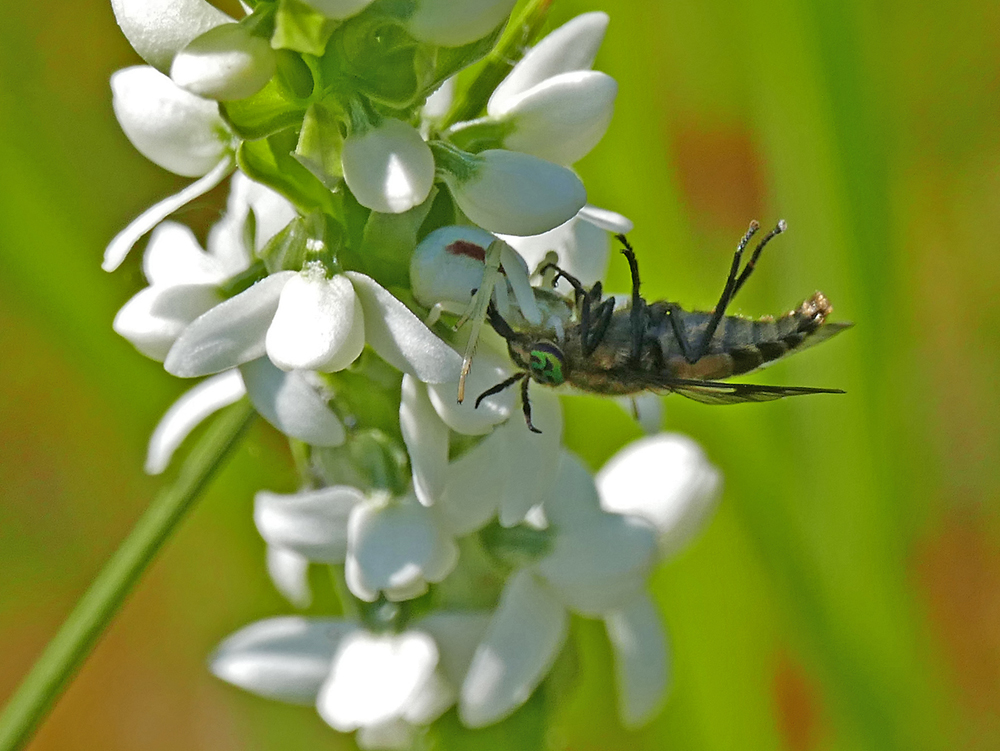
\includegraphics[width=\textwidth]{img/Misumena_vatia_Tabanidae.jpg}
\caption{A female goldenrod crab spider (\emph{Misumena vatia}) with a horse fly (Tabanidae) on \emph{Platanthera dilatata}.}
\label{Misumena_vatia_Tabanidae}
\end{center}
\end{figure}

Nectar thievery is well known among flowers and insects, but a complex
relationship among multiple orchid and insect species has not been
reported from North America. We established that while Noctuidae moths
function as adapted pollinators of \emph{Platanthera dilatata}, they
appear to be nocturnal nectar thieves of two other orchid species
(\emph{Goodyera oblongifolia} and S.\ romanzoffiana) that are diurnally
pollinated by \emph{Bombus} species. Further, \emph{G.\ oblongifolia} is
also visited by a second nectar thief, the geranium plume moth
(\emph{Amblyptilia pica}), which overwinters as an adult and may rely on
this local nectar resource. We also observed a plume moth acting as a
nectar thief on \emph{P.\ dilatata}.

\section{Acknowledgments}

We are grateful to the many people who contributed to this study. Derek
Sikes and Joey Slowik (University of Alaska Museum of the North),
identified difficult insects and spiders, respectively. Bob Biagi,
Robbin McLeod and Bill Dean (\href{https://bugguide.net/}{BugGuide.net}), also identified Bibionidae,
Noctuidae and Syrphidae species, respectively. John Hudson assisted
with additional insect identification and a provided blacklight capture
of Noctuidae moths, and Gwen Balus also identified an additional
Noctuidae. Rita Hassert (The Morton Arboretum), provided essential
library assistance. We are also grateful to Don Kurz and Mary Willson
for reviewing the manuscript, and to Lisa Wallace for comments on the
pollinator network model.

%\bibliography{pollinator_network}

\begin{thebibliography}{27}
\expandafter\ifx\csname natexlab\endcsname\relax\def\natexlab#1{#1}\fi
\expandafter\ifx\csname url\endcsname\relax
  \def\url#1{{\tt #1}}\fi
\expandafter\ifx\csname urlprefix\endcsname\relax\def\urlprefix{{\small URL}
  }\fi

\bibitem[{Ackerman(1975)}]{Ackerman1975}
Ackerman, J.~D.
\newblock 1975.
\newblock Reprocuctive biology of \emph{Goodyera oblongifolia}.
\newblock Madro\~{n}o {\bfseries 23}:191--198.
\newblock \urlprefix\url{http://www.jstor.org/stable/41424024}.

\bibitem[{Ackerman(1981)}]{Ackerman1981}
Ackerman, J.~D.
\newblock 1981.
\newblock Pollination biology of \emph{Calypso bulbosa} var.\
  \emph{occidentalis} (Orchidaceae): a food-deception system.
\newblock Madro\~{n}o {\bfseries 28}:101--110.
\newblock \urlprefix\url{http://www.jstor.org/stable/41424311}.

\bibitem[{Ackerman and Mesler(1979)}]{AckermanMesler1979}
Ackerman, J.~D., and M.~R. Mesler.
\newblock 1979.
\newblock Pollination biology of \emph{Listera cordata} (Orchidaceae).
\newblock American Journal of Botany {\bfseries 66}:820--824.
\newblock \doi{10.1002/j.1537-2197.1979.tb06288.x}.

\bibitem[{Argue(2012{\natexlab{{\em a\/}}})}]{Argue2012a}
Argue, C.~L.
\newblock 2012{\natexlab{{\em a\/}}}.
\newblock The Pollination Biology of North American Orchids: Volume 1: North of
  Florida and Mexico.
\newblock Springer-Verlag, New York.
\newblock \doi{10.1007/978-1-4614-0592-4}.

\bibitem[{Argue(2012{\natexlab{{\em b\/}}})}]{Argue2012b}
Argue, C.~L.
\newblock 2012{\natexlab{{\em b\/}}}.
\newblock The Pollination Biology of North American Orchids: Volume 2: North of
  Florida and Mexico.
\newblock Springer-Verlag, New York.
\newblock \doi{10.1007/978-1-4614-0622-8}.

\bibitem[{Bergum et~al.(2018)Bergum, Cleavitt, and Matthews}]{Bergumetal2018}
Bergum, M., N.~Cleavitt, and D.~Matthews.
\newblock 2018.
\newblock An unexpected visitor.
\newblock Frontiers in Ecology and the Environment {\bfseries 16}:502--502.
\newblock \doi{10.1002/fee.1968}.

\bibitem[{Bieniek et~al.(2012)Bieniek, Bhatt, Thoman, Angeloff, Partain,
  Papineau, Fritsch, Holloway, Walsh, Daly, Shulski, Hufford, Hill, Calos, and
  Gens}]{Bienieketal2012}
Bieniek, P.~A., U.~S. Bhatt, R.~L. Thoman, H.~Angeloff, J.~Partain,
  J.~Papineau, F.~Fritsch, E.~Holloway, J.~E. Walsh, C.~Daly, M.~Shulski,
  G.~Hufford, D.~F. Hill, S.~Calos, and R.~Gens.
\newblock 2012.
\newblock Climate divisions for Alaska based on objective methods.
\newblock Journal of Applied Meteorology and Climatology {\bfseries
  51}:1276--1289.
\newblock \doi{10.1175/JAMC-D-11-0168.1}.

\bibitem[{Bowles and Armstrong(2019)}]{BowlesArmstrong2019}
Bowles, M.~L., and R.~Armstrong.
\newblock 2019.
\newblock Native Orchids in Southeast Alaska.
\newblock
  \urlprefix\url{https://www.naturebob.com/sites/default/files/Bowles-Armstrong-2019-Native-Orchids-in-Southeast-Alaska.pdf}.

\bibitem[{Brown(2006)}]{Brown2006}
Brown, P.~M.
\newblock 2006.
\newblock Wild Orchids of the Pacific Northwest and Canadian Rockies. The
  University Press of Florida.
\newblock The University Press of Florida, Gainesville, Florida.

\bibitem[{Catling(1983)}]{Catling1983}
Catling, P.~M.
\newblock 1983.
\newblock Autogamy in eastern Canadian Orchidaceae: a review of current
  knowledge and some new observations.
\newblock Le Naturaliste Canadien {\bfseries 110}:37--53.

\bibitem[{Catling(1984)}]{Catling1984}
Catling, P.~M.
\newblock 1984.
\newblock Self-pollination and probable autogamy in Chamisso's orchid
  (\emph{Platanthera chorisiana} (Cham.) Reichb.F.
\newblock Le Naturaliste Canadien {\bfseries 111}:451--453.

\bibitem[{Claessens and Seiffert(2017)}]{ClaessensSeiffert2017}
Claessens, J., and B.~Seiffert.
\newblock 2017.
\newblock Significant ant pollination in two orchid species in the Alps as
  adaptation to the climate of the alpine zone?
\newblock Tuexenia {\bfseries 37}:363--374.
\newblock \doi{10.14471/2017.37.005}.

\bibitem[{Darwin(1862)}]{Darwin1862}
Darwin, C.
\newblock 1862.
\newblock The various contrivances by which orchids are fertilised by insects.
\newblock John Murray, London.
\newblock \doi{10.5962/bhl.title.37883}.

\bibitem[{Freudenstein(1997)}]{Freudenstein1997}
Freudenstein, J.~V.
\newblock 1997.
\newblock A monograph of \emph{Corallorhiza} (Orchidaceae).
\newblock Harvard Papers in Botany {\bfseries 1}:5--51.
\newblock \urlprefix\url{http://www.jstor.org/stable/41761525}.

\bibitem[{Gorham(1976)}]{Gorham1976}
Gorham, J.~R.
\newblock 1976.
\newblock Orchid pollination by \emph{Aedes} mosquitoes in {Alaska}.
\newblock The American Midland Naturalist {\bfseries 95}:208--210.
\newblock \doi{10.2307/2424249},
  \urlprefix\url{http://www.jstor.org/stable/2424249}.

\bibitem[{Hapeman and Inoue(1997)}]{HapemanInoue1997}
Hapeman, J.~R., and K.~Inoue.
\newblock 1997.
\newblock Plant-pollinator interactions and floral radiation in
  \textit{Platanthera} (Orchidaceae).
\newblock Pp.\ 432--454 {\em in\/} T.~J. Givnish and K.~J. Sytsma, editors.
  Molecular Evolution and Adaptive Radiation. Cambridge University Press, New
  York.

\bibitem[{Hultén(1968)}]{Hulten1968}
Hultén, E.
\newblock 1968.
\newblock Flora of {Alaska} and neighboring territories.
\newblock Stanford University Press, Stanford, California.

\bibitem[{Inoue(1981)}]{Inoue1981}
Inoue, K.
\newblock 1981.
\newblock Beetle pollination of \emph{Platanthera chorisiana} (Orchidaceae).
\newblock Journal of Japanese Botany {\bfseries 56}:213--218.
\newblock \urlprefix\url{https://ci.nii.ac.jp/naid/10010456333/en/}.

\bibitem[{Inouye(1980)}]{Inouye1980}
Inouye, D.~W.
\newblock 1980.
\newblock The terminology of floral larceny.
\newblock Ecology {\bfseries 61}:1251--1253.
\newblock \doi{10.2307/1936841}.

\bibitem[{Larson and Larson(1990)}]{LarsonLarson1990}
Larson, K.~S., and R.~J. Larson.
\newblock 1990.
\newblock Lure of the locks: showiest ladies-tresses orchids, \emph{Spiranthes
  romanzoffiana}, affect bumblebee, \emph{Bombus} spp., foraging behavior.
\newblock Canadian Field-Naturalist {\bfseries 104}:519--525.

\bibitem[{Larson(1992)}]{Larson1992}
Larson, R.~J.
\newblock 1992.
\newblock Pollination of \emph{Platanthera dilitata} var.\ \emph{dilatata} in
  {Oregon} by the noctuid moth \emph{Discestra oregonica}.
\newblock Madro\~{n}o {\bfseries 39}:236--242.

\bibitem[{Larson and Larson.(1987)}]{LarsonLarson1987}
Larson, R.~J., and K.~S. Larson.
\newblock 1987.
\newblock Observations on the pollination biology of \emph{Spiranthes
  romanzoffiana}.
\newblock Lindleyana {\bfseries 4}:176--179.

\bibitem[{Olesen et~al.(2007)Olesen, Bascompte, Dupont, and
  Jordano}]{Olesenetal2007}
Olesen, J.~M., J.~Bascompte, Y.~L. Dupont, and P.~Jordano.
\newblock 2007.
\newblock The modularity of pollination networks.
\newblock Proceedings of the National Academy of Sciences {\bfseries
  104}:19891--19896.
\newblock \doi{10.1073/pnas.0706375104}.

\bibitem[{Patt et~al.(1989)Patt, Merchant, Williams, and Meeuse}]{Pattetal1989}
Patt, J.~M., M.~W. Merchant, e.~R.~E. Williams, and B.~J.~D. Meeuse.
\newblock 1989.
\newblock Pollination Biology of \emph{Platanthera stricta} (Orchidaceae) in
  Olympic National Park,Washington.
\newblock American Journal of Botany {\bfseries 76}:1097--1106.
\newblock \doi{10.1002/j.1537-2197.1989.tb15093.x}.

\bibitem[{Reeves and Reeves(1984)}]{ReevesReeves1984}
Reeves, L.~M., and T.~R. Reeves.
\newblock 1984.
\newblock Life history and reproduction of \emph{Malaxis paludosa} in
  Minnesota.
\newblock American Orchid Society Bulletin {\bfseries 53}:1880--1291.

\bibitem[{Sheviak~C.(2002)}]{Sheviak2002}
Sheviak~C., J.
\newblock 2002.
\newblock \emph{Platanthera} Richard.
\newblock Pp.\ 551--571 {\em in\/} {Flora of North America Editorial
  Committee}, editor. Flora of North America North of Mexico, volume~26. Oxford
  University Press, New York.

\bibitem[{Zhang et~al.(2014)Zhang, Zhao, and Inouye}]{Zhangetal2014}
Zhang, Y.-W., J.-M. Zhao, and D.~W. Inouye.
\newblock 2014.
\newblock Nectar thieves influence reproductive fitness by altering behaviour
  of nectar robbers and legitimate pollinators in \emph{Corydalis ambigua}
  (Fumariaceae).
\newblock Journal of Ecology {\bfseries 102}:229--237.
\newblock \doi{10.1111/1365-2745.12166}.

\end{thebibliography}


\section{Videos and slide shows}\label{videos}

Below are links to videos and slide shows of insects visiting orchids in the Juneau area. Feel free to download and use however you wish.

\subsection{Bumblebees}
\begin{description}
\item[Video:]  Bumblebees on Western Coralroot Orchids \url{https://vimeo.com/343560365}
\item[Video:]   Bumblebee on White Bog Orchid \url{https://vimeo.com/342178916}
\item[Video:]   Bumblebee on Bog Orchid \url{https://vimeo.com/280660265}
\item[Video:]   Bee mimic and bumblebee on Ladies-tresses Orchid \url{https://vimeo.com/285643040}
\end{description}

\subsection{Butterflies}

\begin{description}
\item[Video:]  Margined White Butterfly on White Bog Orchid  \url{https://vimeo.com/343845001}
\end{description}

\subsection{Dance flies}

\begin{description}
\item[Video:]  Early Coral Root Orchid with Dance Fly \url{https://vimeo.com/337668892} 
\item[Video:]  Dance fly on blunt-leaved orchid (Platanthera obtusata) \url{https://vimeo.com/276573344} 
\end{description}

\subsection{\emph{Dryomyza} fly}

\begin{description}
\item[Video:]  \emph{Dryomyza} fly on Northwestern Twayblade Orchid \url{https://vimeo.com/430921806}
\item[Video:]  \emph{Dryomyza} fly on Northwestern Twayblade Orchid on June 17, 2020 \url{https://vimeo.com/430250286}
\item[Video:]  \emph{Dryomyza} flies on a Northwestern Twayblade Orchid in the rain \url{https://vimeo.com/429783758}
\end{description}

\subsection{Insects}

\begin{description}
\item[Slides:] What comes to a White Bog Orchid \url{https://vimeo.com/435323087} 
\item[Video:]  Insect on Heart-leaved Twayblade Orchid Flower \url{https://vimeo.com/421550015}
\item[Video:]  Insect on a Heart-leaved Twayblade Orchid \url{https://vimeo.com/420923156}
\item[Video:]  Insects coming to a Heart-leaved Twayblade Orchid \url{https://vimeo.com/419786193}
\item[Video:]  Beetle and Flies visit White Bog Orchid \url{https://vimeo.com/280590762}
\item[Video:]  Insects on White Bog Orchid \url{https://vimeo.com/343935517}
March Fly:
\item[Video:]  March Flies on Frog Orchids \url{https://vimeo.com/340916436}
\end{description}

\subsection{Moths}

\begin{description}
\item[Slides:] Noctuidae  Moth visits Rattlesnake Plantain Orchid  \url{https://vimeo.com/443394534}
\item[Slides:] Owlet Moths visit Rattlesnake Orchids July 28, 2020 \url{https://vimeo.com/442730723}
\item[Slides:] Owlet Moth visits to Rattlesnake Orchids \url{https://vimeo.com/442134257}
\item[Video:]  Owlet Moth on a White Bog Orchid \url{https://vimeo.com/348093863}
\item[Video:]  Plume Moth on White Bog Orchid at Buckbean Pond \url{https://vimeo.com/431302940}
\item[Video:]  Plume Moths on Rattlesnake Plantain Orchid \url{https://vimeo.com/288474762}
\item[Video:]  Hawkmoth on White Bog-orchid \url{https://vimeo.com/281908716}
\item[Video:]  Hawkmoth on Bog Orchid July 17 \url{https://vimeo.com/280467246}
\item[Video:]  Noctuidae moth on Orchid \url{https://vimeo.com/279993651}
\item[Video:]  Noctuidae moth on bog orchid \url{https://vimeo.com/279969805}
\item[Video:]  Hawkmoth \& Noctuidae Moths on White Bog-orchid July 20 \url{https://vimeo.com/281101155}
\end{description}

\subsection{Rove beetles}

\begin{description}
\item[Slides \& video:]  Rove Beetles on Twayblade Orchids \url{https://vimeo.com/422039321}
\end{description}

\subsection{Spiders}

\begin{description}
\item[Video:]  The Silver Longjawed Orbweaver hunting on a Slender Bog Orchid \url{https://vimeo.com/436958381}
\end{description}

\subsection{Photography}

\begin{description}
\item[Slides:] Timelapse on White Bog Orchids \url{https://vimeo.com/440357095}
\item[Slides:] Timelapse on White Bog Orchid \url{https://vimeo.com/433273359}
\item[Slides \& video:]  Filming Orchids with the Panasonic DMC FZ200 and FZ300 Cameras \url{https://vimeo.com/421616175}
\end{description}

